% Fundamental packages
\documentclass[11pt,a4paper,twoside]{book}
\usepackage[utf8]{inputenc}
\usepackage[american]{babel}
\usepackage{amsmath}
\usepackage{amsfonts}
\usepackage{amssymb}
\usepackage{graphicx}
\usepackage{algorithm}
\usepackage{setspace}
\usepackage[noend]{algpseudocode}
% margins and general lay-out
%\usepackage[inner=3cm,outer=2cm,top=2.5cm,bottom=2.5cm]{geometry}
\usepackage[inner=2.5cm,outer=2.5cm,top=2.5cm,bottom=2.5cm]{geometry}
\pagestyle{plain}
% fonts (Helvetica) and typographical stuff 

\usepackage[T1]{fontenc}
\usepackage{lmodern} 
\usepackage{textcomp} 
\usepackage{pifont}
\usepackage{csquotes}
\usepackage{bm}

% Setting the font should be done after loading the typographic packages which tend to 
% set a new default font. The microtype package should however be loaded after the font ...
% using san serif helvetica clone
%\usepackage{helvet}
%\renewcommand{\familydefault}{\sfdefault}

% phv is another posibility.
% \renewcommand\rmdefault{phv}
\usepackage{microtype}

% additional packages
\usepackage{booktabs}
\usepackage{pdfpages}
\usepackage{hyperref}
\usepackage{float}
\usepackage{todonotes}
\usepackage{caption}
\usepackage{subcaption}
\usepackage{pdflscape}
\usepackage{rotating}
\usepackage{tablefootnote}

% package to manage citations
\usepackage[backend=bibtex,style=authoryear-comp,sorting=nyt,isbn=false,url=false]{biblatex}
\addbibresource{Bibliography/Bibliography.bib}
\addbibresource{Bibliography/Data.bib}

\DeclareCiteCommand{\citeauthor}
  {\boolfalse{citetracker}%
   \boolfalse{pagetracker}%
   \usebibmacro{prenote}}
  {\ifciteindex
     {\indexnames{labelname}}
     {}%
   \printtext[bibhyperref]{\printnames{labelname}}}
  {\multicitedelim}
  {\usebibmacro{postnote}}
  
% Kill the auto-indent
\setlength\parindent{0pt}

% test package
\usepackage{lipsum}

% Packages for list of symbols and list of abbreviations
%\usepackage[nonumberlist,acronym,toc,nomain]{glossaries}
%\makeglossaries
%\newacronym{SDM}{SDM}{species distribution model}
\newacronym{GLM}{GLM}{generalized linear model}
%An acronym with a glossary entry
\newacronym{ANN}{ANN}{artificial neural network}
 

% new definitions
\newcommand{\expit}{\text{expit}} 
\DeclareMathOperator*{\argmax}{arg\,max}

\DeclareMathOperator*{\argmin}{arg\,min}

\doublespacing
% start of the document
\begin{document}

% include cover page + copyright statement + no pagenumbers
 \pagenumbering{gobble}
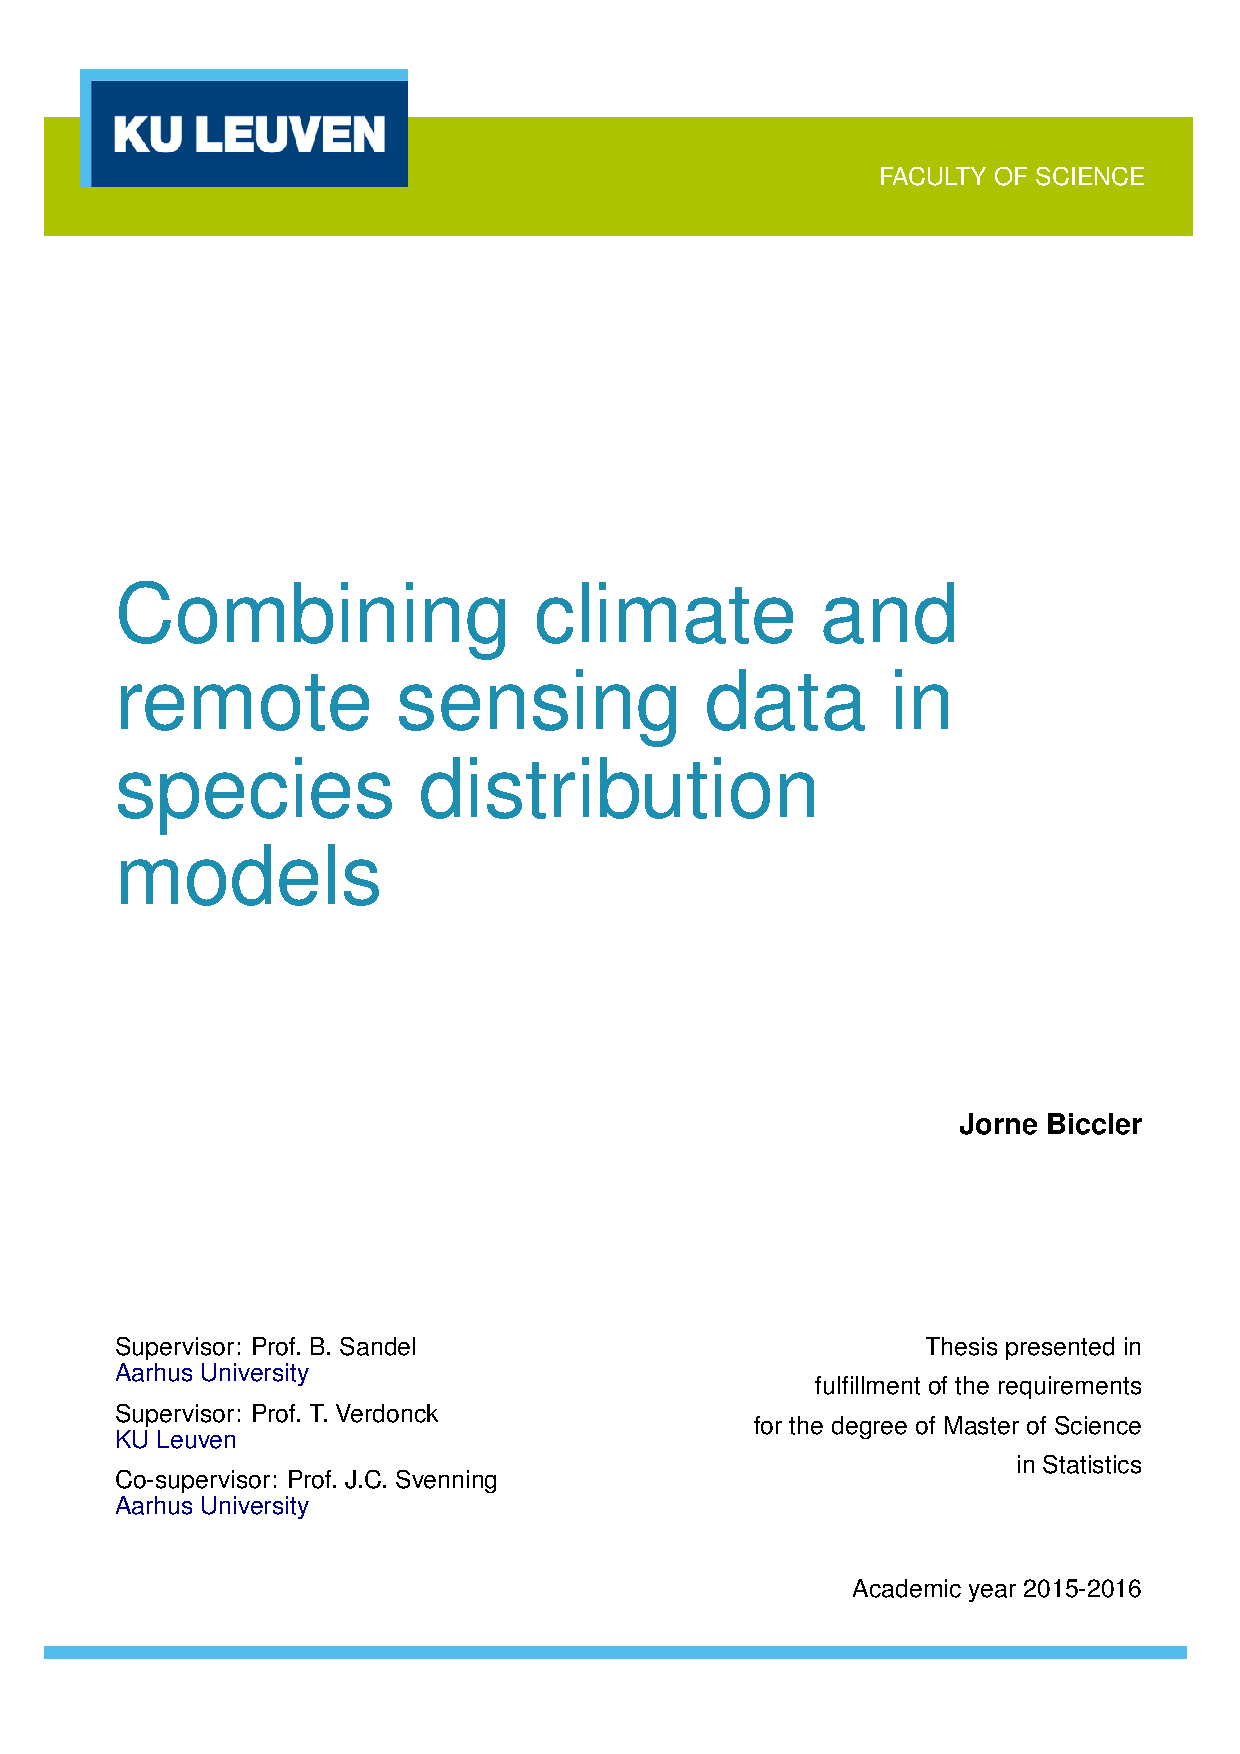
\includepdf[pages={1}]{Cover/TitlePage.pdf}
\clearpage \null \clearpage
\null
\vfill
\copyright~ Copyright by KU Leuven \\

Without written permission of the promotors and the authors it is forbidden to reproduce or adapt in any form or by any means any part of this publication. Requests for obtaining the right to reproduce or utilize parts of this publication should be addressed to KU Leuven, Faculteit Wetenschappen, Geel Huis, Kasteelpark Arenberg 11 bus 2100, 3001 Leuven (Heverlee), Telephone +32 16 32 14 01. \\

A written permission of the promotor is also required to use the methods, products, schematics and programs described in this work for industrial or commercial use, and for submitting this publication in scientific contests.
\cleardoublepage

% frontmatter + roman page numbers
\frontmatter

\chapter{Preface}
\label{ch:Preface}
%In this thesis \gls*{SDM} will be studied. More specifically, we %will investigate \gls*{GLM} and \gls*{ANN}.
% adding * after \gls disables the hyperlinking 
lala
\cleardoublepage
\chapter{Summary}
\label{ch:Summary}

\ldots
something text \\
more text \\
%\printglossary[type=\acronymtype,style=list,title={List of abbreviations}]
\cleardoublepage
\tableofcontents
\listoftodos

% main matter (chapters + appendices
\mainmatter

\chapter{Introduction}
\label{ch:Introduction}
Species distribution modelling (SDM)\footnote{The abbreviation SDM will be used for both the verb, species distribution modelling, and the noun, species distribution model.} concerns the practice of modelling the distribution of a species by use of explanatory variables. Applications include predicting the effect of climate change \parencite{pearson_predicting_2003, pearson_modelling_2004}, predicting the impact of invasive species \parencite{strubbe_predicting_2008}, predicting the occurrence of wildfires \parencite{parisien_environmental_2009}, \ldots \\

Some fundamental ecological concepts are introduced in Chapter \ref{ch:TheEcologicalNicheConcept}. Firstly, the concept of an ecological niche is introduced and the connection with SDMs is made. Secondly, to enhance the understanding of the niche concept some of the assumptions underlying the practice of SDM are discussed. \\

The data-sets and variables that are used in this thesis are described in Chapter \ref{ch:DataCommonlyUsedInSpeciesDistributionModels}. These variables describe either the climate, human influence, elevation, \dots\ at a certain location. Climate data is nearly always used to model the occurrence probability of species. When the goal of a study is to obtain coarse grain predictions over a large spatial extent the use of climate data is certainly justified by ecological theory \parencite{pearson_predicting_2003}. However, if there is interest in predictions over a relatively small extent, e.g.\ when selecting the location of a new national park, fine grain remote sensing data might be useful to distinguish between suitable and unsuitable habitat. \\

Chapter \ref{ch:ClassificationTechniques} introduces a number of modelling techniques that are often used to model the distribution of species. In Section \ref{sec:PresenceAbsenceData} we focus on classical binary classification methods. These methods are directly applicable if there is access to presence-absence data. However, often the data-sets only includes occurrence locations, for example data-sets from natural history musea or citizen science projects are usually of this type. To use presence-only data the classical classification algorithms from Section \ref{sec:PresenceAbsenceData} can be adapted, this is done in Section \ref{sec:ClassificationWithPseudoAbsences}. Another approach is to use one of the algorithms specifically constructed for presence-only data, one of these is introduced in Section \ref{sec:MaximumEntropyModeling}. \\ 
 
In practice a large part of constructing SDMs consists of variable selection. The goal of this thesis is to investigate the performance of multiple model selection methods. An overview of often used methods to deal with large magnitudes of predictors is given in Chapter \ref{ch:ReducingTheNumberOfExplanatoryVariables}. More particularly, we will introduce: 
\begin{itemize}
\item Regularization. 
\item Step-wise selection. 
\item Dimensionality reduction of the explanatory variables. 
\end{itemize}


Although we will introduce the most important concepts and some applications of species distribution modelling, it is not the goal of this thesis to describe every aspect in detail. Instead we refer to \cite{franklin_mapping_2009} who gave an overview of the field of species distribution modelling. Other introductory material include
\cite{guisan_predictive_2000}, \cite{guisan_predicting_2005}, and \cite{elith_species_2009}. An introduction to most of the statistical methodology can be found in \cite{hastie_elements_2009}.























\chapter{The ecological niche concept}
\label{ch:TheEcologicalNicheConcept}
\section{Introduction}
\label{sec:chTheEcologicalNicheConcept:Introduction}
In this chapter the concept of the niche of a species is introduced. The ecological niche of a species can, non-rigorously, be defined as the set of environmental conditions where its reproduction rate is larger than or equal to its mortality rate. Although we will speak of the ecological niche, there are in fact at least three different ``definitions'' that are often used: the Grinnellian niche, the Eltonian niche, and the Hutchinsonian niche. Only a sketch of the niche concept will be given in this section. For a more rigorous description we refer the interested reader to \cite{soberon_grinnellian_2007, soberon_niches_2009}.

\section{Ecological versus geographical space}
In most databases that contain data about species only the location of a presence or absence record is available. Hence, these databases include information about the occurrences or absences in the so-called geographical space. Usually the range of a species' distribution is determined by environmental conditions. We will say that the corresponding variables span the environmental space. It is clear that for each point in the geographical space there is a point in the environmental space. This relation between environmental and geographical space is often called Hutchinson's duality \parencite{colwell_hutchinsons_2009}. A graphical representation of this relation is given in Figure \ref{fig:chTheEcologicalNicheConcept:Niche}. This duality relation is fundamental in SDMs, namely the predictors included in the model are usually assumed to be direct or indirect measures of the variables that span the environmental space. Once a model in the environmental space is constructed the duality relation allows us to make maps of the distribution in the geographical space. \\

\begin{figure}[!htb]
\center
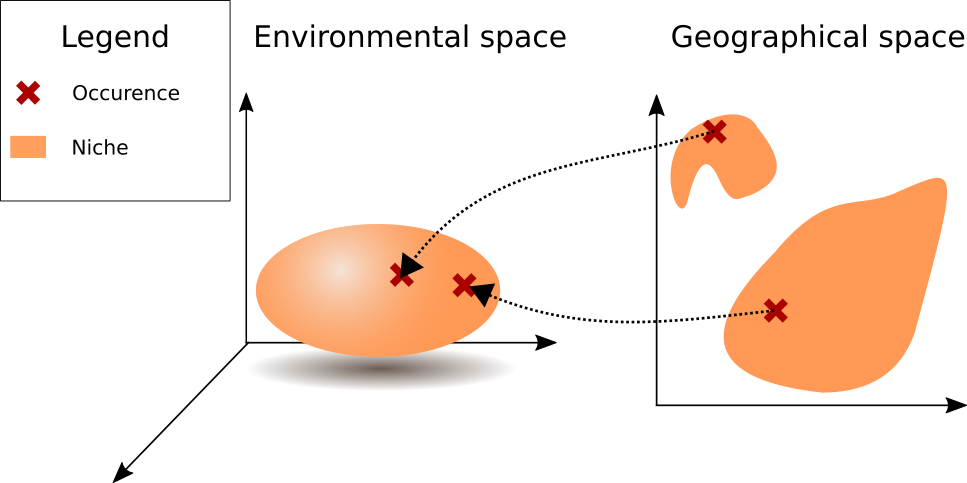
\includegraphics[scale=0.5]{VectorGraphics/Niche.png}
\caption{\label{fig:chTheEcologicalNicheConcept:Niche}Visualization of the duality between environmental and geographical space.}
\end{figure}

In practice a species will often not occur in certain parts of its niche. This can happen because of limited dispersal capabilities of the species, biotic interactions, etc. Such incomplete occupation of the niche leads to the concepts of a fundamental niche and the realized niche. The fundamental niche does not take into account whether or not the species is present, it only represents the suitable conditions. The realized niche is the subset of the fundamental niche where the species is present. These two concepts are depicted in Figure \ref{fig:chTheEcologicalNicheConcept:RealizedNiche}. 
\begin{figure}[!htb]
\center
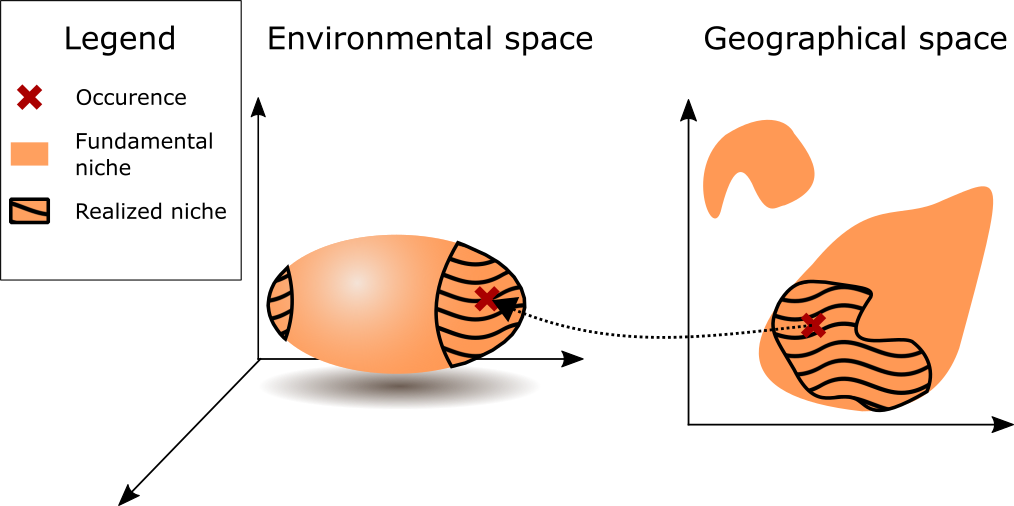
\includegraphics[scale=0.5]{VectorGraphics/RealizedNiche.png}
\caption{\label{fig:chTheEcologicalNicheConcept:RealizedNiche}Visualization of the difference between the fundamental and realized niche.}
\end{figure}

\section{Implicit assumptions when building and using species distribution modles}
\label{sec:chTheEcologicalNicheConcept:NicheEquilibrium}
Before applying SDMs in practice one has to realize that there are some important underlying assumptions. A few of these assumptions are described below. This is done in order to connect the theoretical niche concept to some more practical scenarios and to make the reader aware of the limitations of species distribution modelling. For a more complete overview of the underlying assumptions we refer to \cite{wiens_niches_2009}.\\

Every observed occurrence belongs, by definition, to the realized niche. SDMs are therefore models of the realized niche. If a SDM is used to e.g.\ predict areas prone to invasive species, it is implicitly assumed that, a part of, the realized niche is a good approximation of, a part of, the fundamental niche. Whether this assumption is realistic or not depends on: the species, whether the whole niche has to be approximated or only a part thereof, etc.\\

When data is used to build a model of the realized niche it is assumed that the observed data-points are representative of the niche. In practical settings this is often not the case. We give two examples:
\begin{enumerate}
\item Due to climate change tree species might be found in regions where the current environmental conditions are not included in its niche \parencite{woodward_impact_1990}.
\item The niche of a species usually evolves over time, therefore older observations might not be representative of the current niche \parencite{pearson_predicting_2003}.
\end{enumerate}

Another assumption that is implicitly made in most SDMs is that the effect of biotic interactions is negligible or indirectly captured by other environmental variables. However, in some applications explicitly including biotic interactions has been shown to improve the predictive capabilities \parencite[e.g.][]{heikkinen_biotic_2007}. \\


\section{Spatial scale}
\label{sec:SpatialScale}
From ecological theory we learn that the spatial scale and the extent of the study area play an important role in species distribution modelling \parencite{pearson_predicting_2003, pearson_modelling_2004}. \\

It is often argued that at large scales climate is the main driver of the distribution of species. Land-cover, soil type, and biotic interactions usually only become important when the climate is suitable and hence play a role in fine grain discrimination between suitable and unsuitable conditions. Furthermore, the role of the fine grain drivers might be influenced by the local climatic conditions. \\

The effect of the extent of the study area and the spatial scale are related. When a SDM is applied to a whole continent climate variables will make the biggest contribution to the model. If on the other hand a SDM is developed for a $10\times 10$ km area in Silkeborg the vegetation type might be more important than minor changes in climatic conditions.





\chapter{Data}
\label{ch:DataCommonlyUsedInSpeciesDistributionModels}

\section{Introduction}
To study the performance of the different methods we need data-sets containing on explanatory and outcome data. The different explanatory variables that are used are described in Section \ref{sec:PredictorData}. Given the goals of the thesis we opted for using $33$ different variables. This is more than used in the average SDM and it should be expected that some of them are quite redundant for the species of interest. The species of interest and data-sets that consist of locations where the species was observed to be present or absent are introduced in Section \ref{sec:OutcomeData}.  \\

To process the spatial data R \parencite{RProg} is used as a geographic information system (GIS). To do this we rely on the \textsc{raster} \parencite{raster} and \textsc{sp} \parencite{sp} packages.
\section{Predictor data}
\label{sec:PredictorData}

\subsection{Vegetation Continuous Fields}
The Vegetation Continuous Fields (\Citeauthor[VCF;][]{VCF}) data-set contains values between $0$ and $100$ which are proportional estimates of the tree cover in the cell. Some cells also contain values larger than $100$ which indicate that the cell contains water or that no data is available. Since R has a \textsc{NA} value all the cells with values larger than $100$ are set to \textsc{NA}. The raster is provided in the geographical coordinate system combined with the World Geodetic System 1984 datum (GCS\textunderscore WGS84). The resolution of the VCF raster is $0.00208$ decimal degrees.

\subsection{Bioclimatic variables}
The bioclimatic variables are a set of variables that describe ecologically relevant climate patterns. \todo[inline]{find a citation} The definition of each of the $19$ bioclimatic variables can be found in Table \ref{table:Bioclim}. The bioclimatic variables can be derived from monthly minimum, maximum, and average temperature and precipitation data. Furthermore, it is clear that the BIO05, BIO6, and BIO7 variables are linearly dependent. This linear dependence can be problematic when using classification methods. It is interesting that for some of the methods that we introduce this will lead to no problems while it will for others, see Section \ref{sec:combinations}. \\ 

\begin{table}[htb]
\centering
\begin{tabular}{ll}
\toprule
Variable name & Definition \\ 
\midrule
BIO1 & Annual mean temperature \\
BIO2 & Mean diurnal range (mean of monthly $\left( \text{temp}_{max} - \text{temp}_{min} \right)$) \\
BIO3 & Isothermality $\left( 100 \times \frac{\text{BIO2}}{\text{BIO7}} \right)$  \\
BIO4 & Temperature seasonality $\left(SD(\text{temp}_{avg}) \times 100\right)$ \\
BIO5 & Max temperature of warmest month \\
BIO6 & Min temperature of coldest month \\
BIO7 & Temperature annual range $\left(\text{BIO5} - \text{BIO6}\right)$ \\
BIO8 & Mean temperature of wettest quarter \\
BIO9 & Mean temperature of driest quarter \\
BIO10 & Mean temperature of warmest quarter \\
BIO11 & Mean temperature of coldest quarter \\
BIO12 & Annual precipitation \\
BIO13 & Precipitation of wettest month \\
BIO14 & Precipitation of driest month \\
BIO15 & Precipitation seasonality $\left( \frac{SD( \text{percipitation})}{\text{mean}(\text{percipitaiton})} \right)$ \\
BIO16 & Precipitation of wettest quarter \\
BIO17 & Precipitation of driest quarter \\
BIO18 & Precipitation of warmest quarter \\
BIO19 & Precipitation of coldest quarter \\
\bottomrule
\end{tabular}
\caption{\label{table:Bioclim}Definition of the bioclimatic variables.}
\end{table}

The monthly temperature and precipitation data was obtained from the PRISM database (\cite{daly_knowledge-based_2002}, \citeauthor{PRISM}). The PRISM rasters have a grid cell size of $0.00833$ decimal degrees and the rasters are provided in the GCS\textunderscore WGS84 spatial reference system. \\ 

To calculate the bioclimatic variables we adapted the \textsc{biovars} function from the \textsc{dismo} package \parencite{dismo}. The \textsc{biovars} function from the \textsc{dismo} package does not allow the user to provide a layer of the mean temperature. Instead of using the mean temperature in the calculations it uses the average of the minimum and maximum temperature. Our adaptation does use the mean temperature layers and should be slightly more accurate.

\subsection{Normalized Difference Vegetation Index}
The Normalized Difference Vegetation Index (NDVI) is an index of the amount of vegetation. It is based on measurements of the reflectance in the infra-red and the near infra-red region. The NDVI takes on values between $-1$ and $1$. High values correspond with live green vegetation. The NDVI rasters used in this thesis came from the Global Inventory Modelling and Mapping Studies (GIMMS) and was provided by the University of Maryland Global Land Cover Facility \parencite{pinzon2005satellite, tucker2005extended}. This database contains semi-monthly rasters of the NDVI value for the period 1983-2006. The original rasters had a cell-size of $0.07266$ decimal degrees. These rasters were originally \todo[inline]{cite paper Brody / Svenning on greenes in the US} resampled to $0.04166$ decimal degree rasters and cells with values corresponding to water or with no data available were set to \textsc{NA}. The semi-monthly rasters were then combined such that monthly rasters were obtained. To obtain an average monthly NDVI raster for each month the $24$ NDVI rasters of the different years were averaged. The $12$ resulting monthly NDVI rasters can then be used to calculate a minimum, maximum, and mean NDVI raster.

\subsection{Digital elevation model}
The digital elevation model (DEM) raster \parencite{DEM} contains data on the elevation throughout the US. It is the raster with the highest resolution, more specifically the cell size is $0.000833$ decimal degrees and the raster is provided in the GCS\textunderscore WGS84 spatial reference system. The use of elevation data in SDM is somewhat contested, see e.g.\ \cite{hof_usefulness_2012, oke_distribution_2015}. However, since our main purpose is to test model selection techniques adding a potentially irrelevant predictor should not matter. Furthermore, it is often suggested that other variables directly derived from DEMs, e.g.\ slope, are more ecological relevant \parencite{franklin_mapping_2009}. However, to keep the amount of data in this thesis handleable we will restrict ourselves to the original DEM raster.


\subsection{Land cover}
The land cover data was created from the National Land Cover Databases (NLCD) provided by the US Geological Survey. The NLCD were derived from landsat imagery of 2001 \parencite{vogelmann2001completion}, 2007 \parencite{homer2007completion}, and 2011 \parencite{fry2011completion}. These datasets were then transformed into rasters that utilize the Anderson level 1 classification \parencite{anderson_land_1976}. Eight different land cover classes are used: barren, forest, ice-snow, grassland, urban, water, wetlands, agriculture. For each land cover class-year combination rasters with a cell size of $0.04166$ decimal degrees were created. In order to obtain one raster for each land cover class the three corresponding rasters were averaged. The eight final rasters were then rescaled such that the values of the rasters lie within the interval $[0,1]$. For each land cover class raster the cell values are an estimate of the percentage of the land of this class within the cell. It is interesting that the sum of these rasters equals one, hence there is a linear dependence between the variables.

\subsection{Human Influence Index}
The Human Influence Index (\citeauthor{hii}) raster contains integer values between $0$ and $64$. High values indicate a strong human influence and vice versa. The index is derived from measures of the population density, the amount of roads, the amount of light sources during night-time, etc. The raster was reprojected, see Section \ref{sec:preprocessing}, to the GCS\textunderscore WGS84 spatial reference system and has a cell size of $0.00833$ decimal degrees.

\subsection{Preprocessing of the predictor data}
\label{sec:preprocessing}
In order to speed up computations and facilitate general GIS operations the rasters were, if necessary, reprojected to the GCS\textunderscore WGS84 spatial reference system. The extent and resolution of the rasters were set to be equal to those of the DEM layer. When necessary bilinear interpolation was used. This procedure makes sure that the cells of the rasters line up nicely. A visualization of the whole process can be found in Figure \ref{fig:DataCommonlyUsedInSpeciesDistributionModels:DataScheme}. Once all the data was preprocessed the rasters amount to over $300$ GB of data.

\begin{figure}[!htb]
\centering
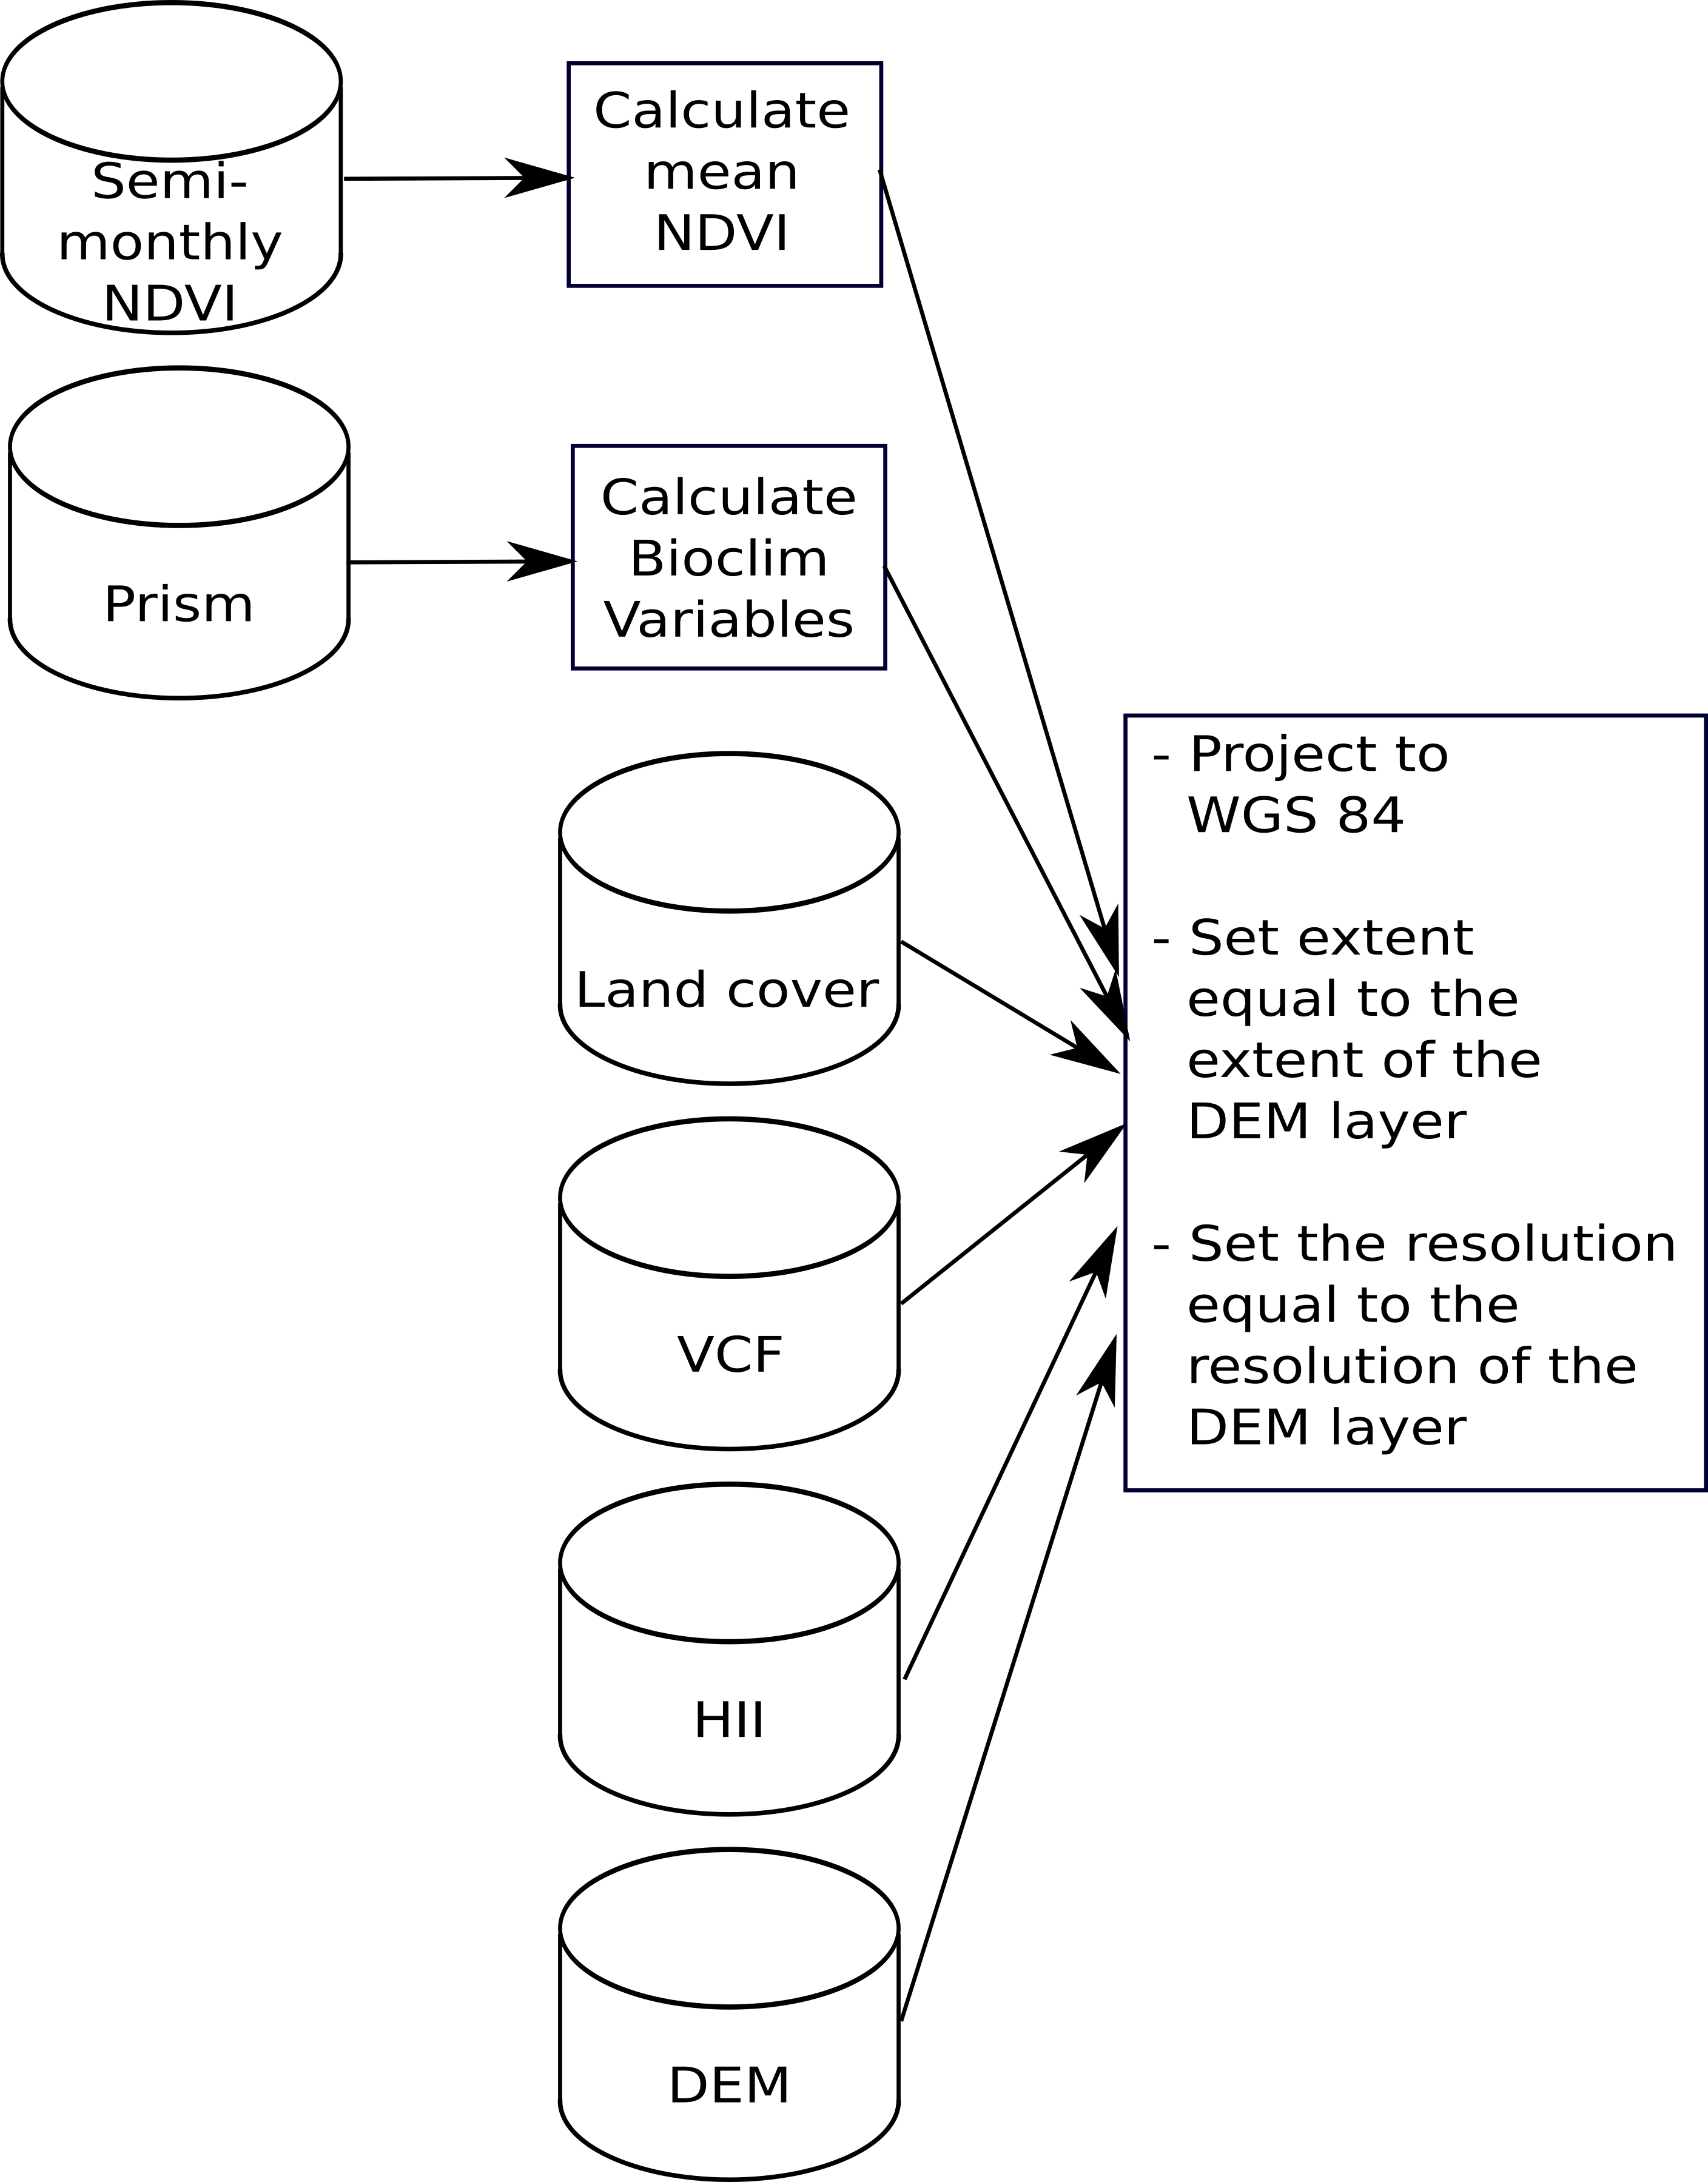
\includegraphics[scale=0.35]{VectorGraphics/DataScheme.png}
\caption{\label{fig:DataCommonlyUsedInSpeciesDistributionModels:DataScheme}Visualization of the preprocessing of the raster data.}
\end{figure}


\subsection{Exploratory analysis of the predictor data}
\label{sec:ExploratoryPredictor}
It might be expected that the relationship between the variables is different in different regions of the contiguous US. To test this we defined four regions, their bounding rectangles can be found in Figure \ref{fig:studyExtent}. To test our suspicions two sets of random points were generated: one with points within the contiguous United States and one that contains points within the West Coast region. For each point the corresponding values of the predictor rasters were extracted. Heat maps of the correlations of the predictor variables can be found in Figures \ref{fig:HeatBGUS} and \ref{fig:HeatBGWC}. A quick inspection of these plots learns that most correlations are approximately equal in the two ranges. There are also some correlations that change quite dramatically, e.g.\ the correlation between the ice-snow land cover class and the NDVI indices. Even though we only report the heat maps of the correlations for the US and the West Coast region similar similar changes can be observed for the other regions. \\

\begin{figure}[!htb]
\centering
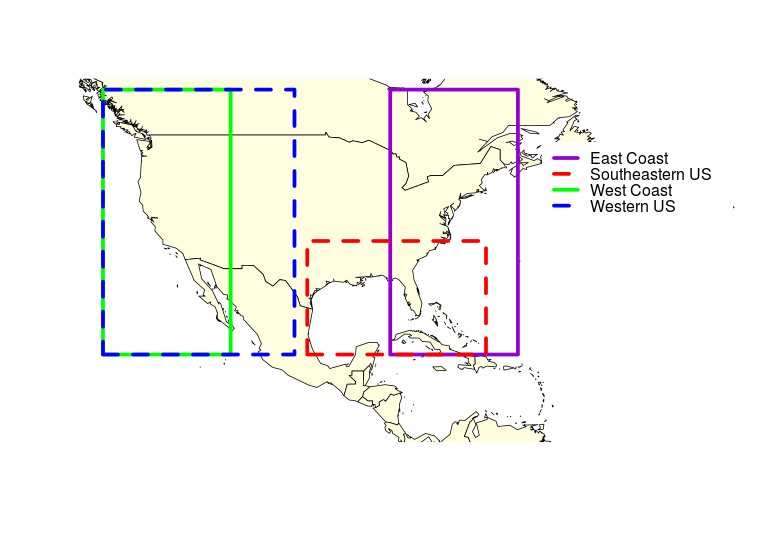
\includegraphics[scale=0.6]{Plots/StudyExtent.png}
\caption{\label{fig:studyExtent}Regions of the contiguous US and their bounding rectangles.}
\end{figure}

It is interesting to note that the rank of the predictor data matrix of the random points is $32$. This is rather surprising since BIO7 is a linear combination of BIO5 and BIO6 and the land cover variables should sum to a constant. Hence one would expect that the rank is smaller or equal to $33-2 =31$. A closer inspection leads to the conclusion that some small rounding errors in the creation of the land cover rasters ``remove'' the linear dependence. This ``near linear dependence'' also becomes clear when we look at the singular values of the scaled data matrix. The three smallest are $0.2139771, 0.000002,$ and $0$, for all practical purposes this means that there are two redundant variables.\\

\begin{landscape}
\thispagestyle{empty}
\null
\vskip 0.6cm

\begin{figure}[!htb]
  \centering
  \makebox[\textwidth][c]{%
    \begin{minipage}{.90\textwidth}
    \centering
    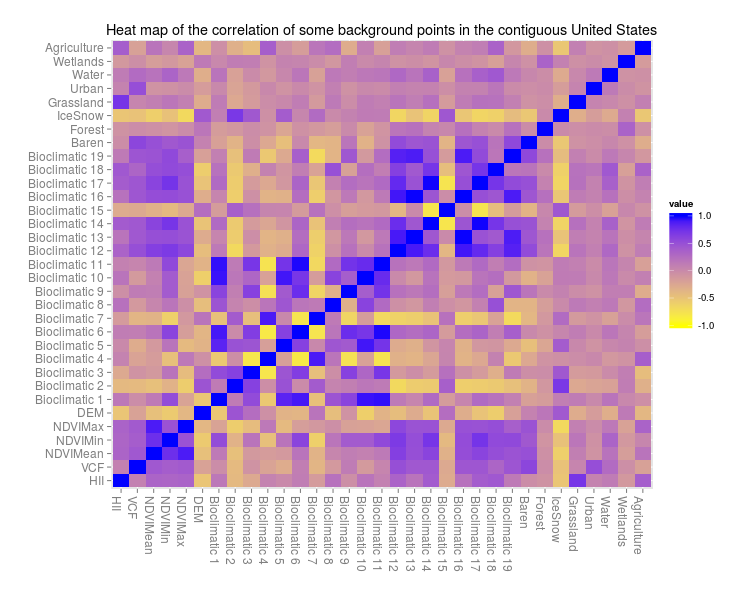
\includegraphics[width=\textwidth]{Plots/CorPlotUS.png}
    \caption{\label{fig:HeatBGUS}Heat map of the correlations in the contiguous US.}
    \end{minipage}
    \begin{minipage}{.90\textwidth}
    \centering
    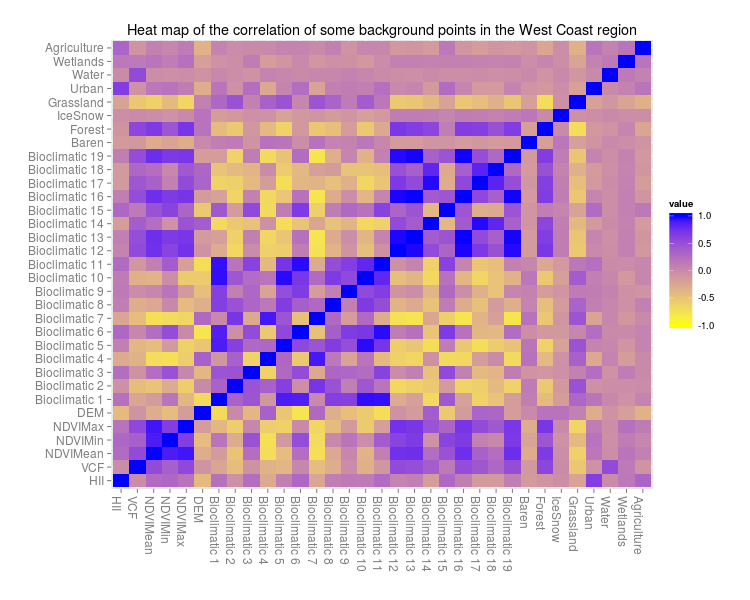
\includegraphics[width=\textwidth]{Plots/CorPlotBGWC.png}
    \caption{\label{fig:HeatBGWC}Heat map of the correlations in the West Coast region.}		\end{minipage}%
}
\end{figure}
\end{landscape}


\section{Outcome data}
\label{sec:OutcomeData}
\subsection{Species considered}
The species that will be studied can be found in Table \ref{table:Species}. These species were selected so that different regions in the US are represented. This was done because, as we saw in Section \ref{sec:ExploratoryPredictor}, the relationship between the different predictors can be different in different regions. The extent of the distributions are quite different across the selected species. For example, the copperhead snake is spread throughout a large part of the US while the Sequoia sempervirens only occurs in a small strip of land stretching from Southern California to Southern Oregon. Finally, the set of selected species consists of five plant and five animal species. Selecting both plant and animal species was done because it seems reasonable that the including fine grain predictors will lead to a larger increase in predictive performance of the classification models when the species is stationary.\\

Since the study areas considered are relatively large it can be expected that the bioclimatic variables will be the most important variables, see Section \ref{sec:SpatialScale}. Since we are specifically interested in dealing with redundant variables it should, as stated earlier, not really matter whether or not only the bioclimatic variables are important.

\begin{sidewaystable}[ph!]
\centering
\begin{tabular}{l l c c c c c }
\toprule
Species & Common name & US & West Coast & East Coast & Western US & Southeastern US \\
\midrule
Aesculus glabra & Ohio buckeye  &  \ding{51} \\
Juniperus osteosperma & Utah juniper  & & &  \ding{51}\\
Quercus ilicifolia & bear oak  & & &  \ding{51}  \\
Salix caroliniana & coastal plain willow  &  \ding{51}  \\
Sequoia sempervirens & coast redwood & &  \ding{51}  \\
\\
Agkistrodon contortrix Linnaeus & copperhead snake   &  \ding{51}  \\
Geomys pinetis Rafinesque & southeastern pocket gopher  &&&& &  \ding{51}  \\
Pituophis catenifer catenifer & Pacific gopher snake  &  &  \ding{51}  \\
Sorex pacificus & Pacific shrew &  &  \ding{51}  \\
Sylvilagus nuttallii & mountain cottontail  & & &  &  \ding{51}  \\
\bottomrule
\end{tabular}
\caption{\label{table:Species}The different species studied and their study extent.}
\end{sidewaystable}

\subsection{Global Biodiversity Information Facility}
The presence-only data came from the Global Biodiversity Information Facility (GBIF) database. This database contains data from other smaller presence-only databases. Examples include data from citizen science projects (e.g.\ the iNaturalist project) or herbariums (e.g.\ The New York Botanical Garden Herbarium). These data sources are quite prone to errors. Citizen science data is usually provided by non-experts and misidentifications are quite likely. Even data collected by experts can be irrelevant for our purposes, for example herbarium data often includes specimens located inside botanical gardens etc. GBIF data tends to contain a lot of duplicated observations. Hence, before using the data some data-cleaning was performed. Finally, because the predictors were recorded quite recently we decided to restrict ourselves to observations obtained from the 1980s onward. To some extent this prevents the situation where the current predictor values have changed recently, e.g. due to deforestation.\\

\subsection{Forest Inventory and Analysis data}
The presence-absence data of the plant species was obtained from the The United States Forest Service Forest Inventory and Analysis (FIA) database. The data from this database consists of plot locations and all the tree species observed within each plot are recorded. The reported coordinates of the plots are, for privacy reasons, slightly distorted.\\ 

The sampling design that is used in the construction of this database changed in 1999 and details can be found in \cite{fiamanual}. By 2004 the new sampling design was implemented in nearly all the states of the contiguous US. The exceptions to this are New Mexico, Oklahoma, and Wyoming for which the new design was implemented in 2005, 2008-2009, and 2011. In each state at least $10\%$ of the plots are sampled each year. By using a time-frame of $10$ years we ensured that each plot site was sampled. More particularly, the time-frame that was used is 2004-2014. Since the sampling in New Mexico, Oklahoma, and Wyoming started later than 2004 these states were under-sampled. States in the Eastern US tend to have a sample intensity larger than $10\%$ and some plots were sampled multiple times. Plots that were sampled multiple times were replaced by new observations. If a plot contained the species of interest at least once the species was said to have been present, otherwise it was absent in the plot. It might be interesting to use modelling methods that allow for a sampling design correction. However, this would lead us astray and the sampling design will not be corrected for in this thesis.\\

Finally, all of the sampled plots are contained within forested areas. This implies that lone standing trees were not observed.

\subsection{Data preparation}
In order to build the necessary models the predictor values corresponding to the presence or absence locations are needed. For certain locations some of the rasters contained a \textsc{NA} value. These locations were removed before the models were constructed. The number of occurrences for each species can be found in Table \ref{table:NrObs}. The total number of plots contained within each region can be found in Table \ref{table:PlotsRegion}.

\begin{table}
    \begin{minipage}{.5\linewidth}
      
      \centering
        \begin{tabular}{lcc}
            \toprule
            Species & GBIF & FIA \\
            \midrule
Aesculus glabra & 126 & 177 \\
Juniperus osteosperma & 230 & 4131\\
Quercus ilicifolia & 98 & 62 \\
Salix caroliniana &  68 & \\ 
Sequoia sempervirens &  & 206 \\
\\
Agkistrodon contortrix Linnaeus & 1426 & \\
Geomys pinetis Rafinesque & 53 & \\
Pituophis catenifer catenifer & 232 & \\
Sorex pacificus  & 141 & \\
Sylvilagus nuttallii & & \\
            \bottomrule
        \end{tabular}
        \caption{\label{table:NrObs}Number of occurrence observations.}
    \end{minipage}%
    \qquad
    \begin{minipage}{.5\linewidth}
      \centering
        \begin{tabular}{lcc}
        \toprule
        Region & Number of plots \\
        \midrule
            US & 287860 \\
            West Coast &  82184 \\
            East Coast &  42029 \\
            Western US &  144436 \\
            \bottomrule
        \end{tabular}
        \caption{\label{table:PlotsRegion}Number of plots within the regions.}
    \end{minipage} 
\end{table}






\chapter{Classification techniques}
\label{ch:ClassificationTechniques}

\section{Introduction}
This chapter deals with the statistical foundations of species distribution modelling. Since it is impractical to list all the available methods that are used we restrict ourselves to the most popular or fundamental ones. In the last 10 years a lot of research has focused on the performance of these different algorithms \parencite[e.g.][]{elith*_novel_2006,segurado_evaluation_2004}. The results of these studies were taken into account when the methods that are used were selected.

\section{Presence-absence data}
\label{sec:PresenceAbsenceData}

In this section some important and often used methods to classify binary data are reviewed. First of all, the outcome, $y_i$, of observation $i$ indicates whether a species occurs, $y_i = 1$, or is absent, $y_i=0$. We denote the vector of explanatory variables as $\bm{X}$. The general form of the models used in this section is:
\begin{equation}
\label{FundEq}
P(Y=1|\bm{X} = \bm{x}) = f(\bm{x}; \bm{\gamma}).
\end{equation}
In this representation $f(\cdot;\cdot)$ is a function parametrized by $\bm{\gamma}$. The main differences between the techniques introduced below are the functional form of $f(\cdot;\cdot)$ and the loss function that is minimized.

\subsection{Logistic regression}
Perhaps the most fundamental modelling technique for binary data is logistic regression. In logistic regression the log odds ratio of the probability of an occurrence is modelled as a linear function of the covariates. Hence, the model can be depicted as \[\log \left( \frac{P(Y=1|\bm{X} = \bm{x})}{P(Y=0|\bm{X} = \bm{x})} \right)= \gamma_0 \bm{x}^t \bm{\gamma}.\]
It is easy to show that this model can be written in the form used in Equation \ref{FundEq}. More specifically, if we define $\expit(\cdot) = \frac{\exp(\cdot)}{1+\exp(\cdot)}$ we get \[f(\bm{x};\bm{\gamma}) = \expit(\gamma_0 + \mathbf{x}^t\bm{\gamma}).\] Usually the coefficients of a logistic regression model are obtained by using maximum likelihood estimation (MLE). Obtaining the MLE $\widehat{\bm{\gamma}}$ corresponds with solving the following maximization problem:
\[\widehat{\bm{\gamma}} = \argmax_{\bm{\gamma}} \sum_{i=1}^{N} \left\lbrace y_i \log{f(\bm{x}_i;\bm{\gamma})}  + (1-y_i)\log{f(\bm{x}_i;\bm{\gamma})}  \right\rbrace.\] 
When one multiplies this log-likelihood function by minus one we get a loss function that is often called the cross-entropy. For more information about logistic regression and numerical optimization techniques for obtaining the MLE we refer to \cite{agresti_categorical_2013} and \cite{mccullagh_generalized_1999}. \\

The main advantages of logistic regression models are that they are relatively simple to implement, interpret, etc. This simplicity is also its greatest disadvantage. In particular, when modelling the distribution of a species there is often no a priori knowledge of the shape of the response curves.

\subsection{Generalized additive models}
\label{sec:GAM}
In standard logistic regression a linear systematic component is used. It is easy to extend logistic regression models to include non-linear systematic components. However, the functional form of the log odds ratio might not be known by the researcher and hence a non-parametric (or semi-parametric) modelling technique can be useful. When the distribution of the outcome belongs to the exponential family generalized additive models (GAMs) are one possible class of non-parametric (or semi-parametric) models. In the case of a Bernoulli distribution the resulting GAM is sometimes called an additive logistic regression model and has the form:
\begin{equation}
\label{GAMs}
\log \left( \frac{P(Y = 1|\bm{X} = \bm{x} )}{P(Y=0|\bm{X} = \bm{x})} \right) = \gamma_0 + f_1(x_{1}) + \dots + f_p(x_{p}).
\end{equation}
In this representation the $f_k(\cdot)$'s are certain smooth functions. Again one can write this model in the form of Equation \ref{FundEq}:
\[f(\bm{x};\bm{\gamma}) = \gamma_0 + f_1(x_{1}) + \dots + f_p(x_{p})\] 
There is a multitude of popular ways to specify the $f_k(\cdot)$'s \parencite{wood_generalized_2006, hastie_generalized_1990}. We will follow \cite{wood_generalized_2006} and \cite{wood_gams_2002} and focus on using cubic smoothing splines to represent the $f_k(\cdot)$'s. \\

GAMs are most often fitted by using MLE. In order to restrict the ``wiggliness'' of the smoothing functions in model \ref{GAMs} one can add a penalization term to the likelihood function. An example of such a ``wiggliness'' penalty is:
\[\sum_{j=1}^p \lambda_j \int_{x_{j(1)}}^{x_{j(n)}} \{f^{(2)}_j(x) \}^2dx.\]
In this penalization term the $x_{j(1)}$ (resp.\ $x_{j(n)}$) is the smallest (resp.\ largest) value of the $j$'th covariate. Furthermore, it can be shown that, in a class of sufficiently smooth functions, the minimizer of
\[- \sum_{i=1}^{N} \left\lbrace y_i \log{f(\bm{x}_i;\bm{\gamma})}  + (1-y_i)\log{f(\bm{x}_i;\bm{\gamma})} \right\rbrace + \sum_{j=1}^p \lambda_j \int_{x_{j(1)}}^{x_{j(n)}} \{f_j^{(2)}(x)\}^2 dx\]
is a natural cubic spline with knots at the $n$ covariate values. The two limiting cases, $\lambda = 0$ and $\lambda = \infty$, are interesting. If $\lambda = 0$ an interpolating spline is optimal, while when $\lambda \to \infty$ the solution converges to the linear logistic regression solution. Finally, fitting GAMS with natural cubic splines as smoothing functions is, compared to most other smoothers used in GAMS, computationally efficient.\\

In practice we have to select the penalization parameters, this is usually done by using cross-validation. Because the fitting procedures for GAMs are often computationally intensive usually the closely related generalized cross-validation (GCV) is used \parencite{wood_gams_2002}. Finally, since $\lambda = \infty$ still allows a first order fit, it can be interesting to perform additional model selection. Although variable selection is the topic of Chapter \ref{ch:ReducingTheNumberOfExplanatoryVariables} we mention that it is possible to introduce an extra penalization term that leads to an automatic variable selection technique \parencite{marra_practical_2011}, i.e.\ might remove a predictor from the model. This approach is implemented in the \textsc{mgcv} R package \parencite{mgcv}. \\

Finally, up till now only univariate splines have been considered, if interaction terms are to be included one can use e.g.\ thin plate splines. However, using multidimensional splines usually results in a computationally intensive fitting procedure. Finally, for a more applied review of the use of GAMs in species distribution modelling we refer to \cite{guisan_generalized_2002}.

\subsection{Artificial neural networks}
Artificial neural networks (ANNs) are a non-linear modelling technique. We refer to \cite{bishop_neural_1995} for an introduction to the general methodology and some of the technical details. The terminology used in the ANN literature is slightly different than in the standard statistical literature. More particularly, the explanatory variables are usually called the input features. Furthermore, an ANN consists of so-called ``layers'' of ``neurons'. The first layer is called the input layer and consists of one neuron for each variable. In each successive layer the output of the corresponding neurons is the result of applying an activation function, $g(\cdot)$, to a linear combination of the values from the previous layer. The coefficients of these linear combinations are called the weights of the ANN. These weights are the parameters one can tune. The process of feeding the values of the previous layer into the next is repeated up to the last layer which is called the output layer. The layers that are neither the input nor output layer are called hidden layers. A graphical representation of an ANN with one hidden layer can be found in Figure \ref{fig:chClassificationTechniques:ANN}.\\

\begin{figure}[!htb]
\centering
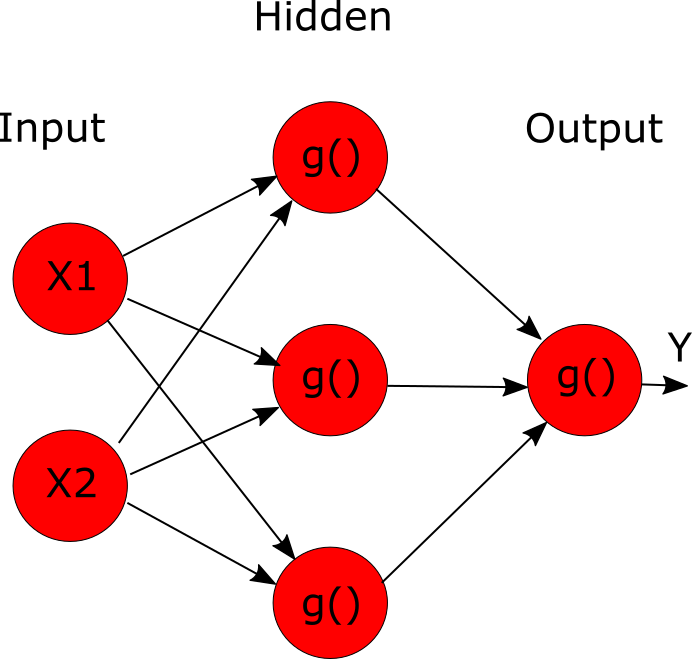
\includegraphics[scale=0.3]{VectorGraphics/ANN.png}
\caption{\label{fig:chClassificationTechniques:ANN}Visualization of a feed-forward neural network with one hidden layer.}
\end{figure}

From here on we will denote the vector of all the weights as $\bm{\gamma}$. As usual, the estimated weights are obtained by minimizing a loss function. When ANNs are applied to classification problems often either the squared loss, $L(\bm{y};\bm{\gamma}) = \sum_i (y_i - f(\bm{x}_i;\bm{\gamma}))^2$ or the cross-entropy, $L(\bm{y};\bm{\gamma}) = - \sum_i \left[ y_i \log \{ f(\bm{x}_i;\bm{\gamma})\} + (1-y_i)\log \{f(\bm{x}_i;\bm{\gamma})\}\right]$ is used. We will use the cross-entropy since it is closely related to the likelihood of a Bernoulli distribution and hence more in line with the other techniques. To minimize the loss criterion, often backpropagation \parencite{rumelhart_learning_1986} is used in combination with a numerical optimization algorithm, e.g.\ steepest descent. \\

It is easy to see that logistic regression can be seen as an ANN with: no hidden layers, the expit function as the activation function of the output layer, and the cross-entropy loss.\\

The biggest strength of ANNs is that, under some regularity constraints, they can approximate any continuous function arbitrarily well \parencite{hornik_multilayer_1989}. Some disadvantages include:
\begin{itemize}
\item Selecting an optimal number of layers and neurons is far from trivial.
\item The loss-function often has multiple local minima.
\item Different numerical optimization methods often lead to different solutions.
\item Fitting large neural network architectures can be computationally infeasible.
\item The backpropagation algorithm cannot be used in combination with non-differentiable penalty functions, e.g.\ the lasso penalty (see Section \ref{sec:Lasso}).
\item The fitted parameters can be sensitive to the initial weights.
\item The obtained model seems like a ``black-box'', i.e. there is often no easy way to interpret the parameters and the effect of different predictors.
\end{itemize}
Some of these disadvantages can be, partially, overcome by using e.g.\ weight decay, averaging networks, early stopping, pruning, \dots\ Weight decay is also referred to as $L_2$ regularization and is described in Section \ref{sec:L2Regularization}. Averaging networks boils down to using different sets of initial values, fitting the same network structure for each set, and then combining these into one model \parencite{ripley_pattern_2009}. The \textsc{caret} package \parencite{caret} provides an implementation of averaged neural networks based upon the \textsc{nnet} package \parencite{nnet}.


\subsection{Tree based methods}
In this section some tree based methods are introduced.  The section starts with a short explanation of decision trees. Afterwards boosting is introduced as a method to deal with some of the shortcomings of decision trees.

\subsubsection{Decision trees}
\label{sec:DecisionTrees}
Tree based methods are a class of algorithms that partition the input space into rectangular regions. The same predicted value is then assigned to all observations within a certain region. In the context of SDMs we can interpret this as partitioning the environmental space into rectangles. Each of these rectangles is then labelled as being part of the niche or not. To obtain such rectangles we start by splitting the input space into two regions along one variable. The variable and the value that is used to obtain this split is selected in such a way that the loss function of interest is minimized. In the following steps either the algorithm stops if some stopping criterion is met or the obtained sub-regions are split into smaller sub-regions. After the tree is grown usually a winner takes all approach is applied to obtain the label for each region. Thus, if a region contains mainly presences its predicted class will be the presence class, otherwise it will be labelled as a region containing absences. Finally, the number of nodes $J$ of a tree is defined as the number of splits $+1$. A visualization of a partitioning obtained bys using a classification tree is given in Figure \ref{fig:chClassificationTechniques:CART}. \\

\begin{figure}[!htb]
\centering
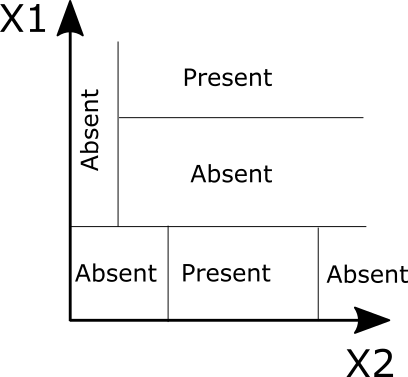
\includegraphics[scale=0.5]{VectorGraphics/CART.png}
\caption{\label{fig:chClassificationTechniques:CART}Visualization of a classification tree in a two dimensional input space.}
\end{figure}

Unless a stopping criteria is specified this approach would lead to over-fitting. More particularly we would end up with as many regions as there are observations. Hence, the algorithm is usually stopped when no new splits can be found that decrease the loss by some pre-specified amount. Another possible stopping criterion is to stop the algorithm once a certain number of splits is reached. As usually we opt for using the cross-entropy as the loss function. Finally, we note that there are many variations to the algorithm sketched above.

The most important advantages of decision trees include:
\begin{itemize}
\item Complex interaction effects can easily be modelled.
\item Small decision trees are easily visualized.
\item Decision trees usually perform relatively well even when no variable selection was applied.
\item The idea underlying decision trees is quite intuitive.
\item Decision trees are invariant under monotonic transformations of the predictors.
\end{itemize}

Some of the disadvantages of using decision trees include:
\begin{itemize}
\item Decision trees usually have a large variance
\item Categorical variables with a lot of classes can lead to computational problems.
\end{itemize}

\subsubsection{Boosting}
\label{sec:Boosting}
In order to combat the large variance of decision tree boosting was introduced. The overview of boosting presented in this section is largely based on \cite{elith_working_2008} and \cite{friedman_additive_2000}. \cite{elith_working_2008} gave an applied working guide to boosted regression trees while \cite{friedman_additive_2000} gave a theoretical explanation of boosted regression trees.\\

An ensemble of different classifiers is sometimes useful to obtain improved classifiers. This is what is done in boosted classification trees. Boosting can be described as creating a sequence of models such that the $i$'th model focusses on correctly classifying observations that were misclassified by the $i-1$ previous models. The corresponding algorithm then takes the following form:\\
\begin{enumerate}
\item Construct a classifier.
\item Classify the observations.
\item Assign large weights to wrongly classified observation and vice versa for correctly classified observations. 
\item Fit a classifier on the weighted data-set.
\item Create a new classifier by adding the the new and old classifiers, usually the new classifier is shrunken by multiplying it with a regularization parameter.
\item Stop if some stopping criteria is met, otherwise use the new classifier obtained in step 5. and repeat from step 2. onwards.
\end{enumerate}

In order to avoid over-fitting one can use a new subsample of the full data-set in each iteration of the algorithm. When combining boosting with classification trees it is recommended that the subsamples have a sample size in between $0.5$ and $0.75$ times the size of the full dataset \parencite{elith_working_2008}.\\

Another popular ensemble method that is used in combination with decision trees is the Random Forest (RF) method. In most cases RFs perform slightly worse than boosted classification trees \parencite{hastie_elements_2009} and we will not consider them in this thesis.\\

A disadvantage of boosted classification trees is that they are not as easily visualized / interpreted as normal classification trees. Secondly, there are quite a few tuning parameters, namely the depth of the trees $J$, the regularization term, and the number of trees. However, \cite{hastie_elements_2009} note that using $J \in \{4,\dots,8\}$ usually leads to the best performing models, additionally they observed that the specific value of $J$ in this set has little effect on the performance of the classifier. Hence, cross validation will be used to obtain optimal values for the learning rate and the number of trees.\\

Finally, although we described boosting for classification trees the same idea can be readily applied to other classification algorithms. Furthermore, boosted classification trees seem to include a form of internal variable selection, i.e.\ the performance of this method usually doesn't degrade a lot when irrelevant predictors are present. We will use the implementation provided by the \textsc{gbm} package \parencite{gbm}.

\section{Presence-only data}
\label{sec:PresenceOnlyData}
Instead of having access to presence-absence data it happens quite often that only presence data is available. Since the previously described classification techniques need binary data they can not immediately be used with presence-only data. In Section \ref{sec:IPP} the inhomogeneous Poisson process (IPP) is introduced. Presence-background classification is introduced in Section \ref{sec:ClassificationWithPseudoAbsences}. Finally, in Section \ref{sec:MaximumEntropyModeling} Maximum Entropy \parencite[MaxEnt;][]{phillips_maximum_2006,phillips_modeling_2008} is concisely described. \\ 

Although we will not consider it we note that there is another interesting way to use regression models in combination with presence-only data. \cite{ward_presence-only_2009} used the EM algorithm \parencite{dempster_maximum_1977} in combination with regression models. Although this leads to an elegant and rigorously motivated method of fitting regression models, the prevalence of the species needs to be known, or estimable, which is nearly never the case.

\subsection{Poisson point processes}
\label{sec:IPP}
First of all, all the measure theoretic machinery involved in point processes is blatantly ignored in this section. We denote the study area of interest by $S$. Usually $S$ corresponds to an area preserving projection of the earth and therefore our focus is on $S\subset \mathbb{R}^2$. A point process is a random variable $\bm{X}$ that consists of points $u_i \in S$, hence $\bm{X} =  (u_1,\ldots,u_n)$. In the presence-only scenario the $\bm{X}$ variable equals the locations where an occurrence was reported. One popular point process is the inhomogeneous Poisson point process. Before giving a non-rigorous definition of the IPP we define the intensity of a point process as a function $\lambda(\cdot): S \to \mathbb{R}_+$ for which $\int_B \lambda(u)du < \infty,\; \forall$ bounded $B \subset S$. The random variable $\bm{X}$ is said be an IPP if $\forall$ bounded $ B \subset S$:
\begin{enumerate}
\item The number of observed points within $B$, $N(B) = \# (X \cap B)$, follows a Poisson distribution with mean $\Lambda(B) = \int_B \lambda(u)du.$
\item Given the number of observed points within $B$, $N(B)$, the elements of $X$ within $B$ are i.i.d. distributed with density $\frac{\lambda(u)}{\Lambda(B)}.$
\end{enumerate}
The first part of the definition implies that the the expected number of observations in a small area surrounding a point is approximately equal to the intensity, assuming it is a continuous function, multiplied by size of the area. \\

In order to obtain a parametric model of an IPP the intensity is usually modelled as a function of the covariates $\bm{z}(u)$ observed at the location $u$. A popular model is the log linear model: 
\begin{equation*}
\label{eq:Intensity}
 \lambda(u) = \exp (\gamma_0  + \bm{\gamma}^t\bm{z}(u) ). 
\end{equation*}
It is interesting to note that the intercept term, $\gamma_0$, only affects the expected number of points but not the configuration of the points in $S$. When we use $C$ to denote a rest term that is independent of the parameters, the likelihood function becomes:
\begin{equation*}
\label{eq:IPPlikelihood}
\begin{aligned}
l(\bm{x};\bm{\gamma}) &= \log \left( \prod_{i=1}^n \frac{\lambda(u_i)}{\Lambda(S)} \frac{ \Lambda(S)^n \exp (-\Lambda(S))}{n!}\right)  \\ 
&= \sum_{i=1}^n \left\lbrace \gamma_0 + \bm{\gamma}^t\bm{z}(u_i) \right\rbrace - \int_S \exp (\bm{\gamma}^t\bm{z}(u)) du  + C.
\end{aligned}
\end{equation*}
The difficulty of using MLE in combination with IPP models is approximating the integral. For an overview of different methods to obtain the MLEs and a more complete treatment of spatial point processes we refer to \cite{moller_modern_2007}.

\subsection{Classification with pseudo-absences}
\label{sec:ClassificationWithPseudoAbsences}
\todo[inline]{discuss effect of using PCA on background vs occurrence data}
One of the older techniques to deal with presence-only data consists of generating so-called pseudo-absence or background points. The original motivation of this technique is that by uniformly sampling $n_0$ points in the geographical space $S$ one obtains a representation of the available habitat in the study region \parencite{pearce_modelling_2006}. The available habitat is then contrasted with the locations where a presence was observed by using standard classification methods. In practice one has to decide on the number of pseudo-absences that should be used and whether or not the pseudo-absences should be weighted \parencite{barbet-massin_selecting_2012}.\\

Another, more rigorous, way to justify the pseudo-absence method is by using the IPP model. \cite{warton_poisson_2010} were the first to note the connections between fitting an IPP model and fitting logistic regression models with pseudo-absences. \cite{fithian_finite-sample_2013} further refined these equivalences and also considered the situation when the model is misspecified. We follow the derivation given by \cite{fithian_finite-sample_2013}.\\

First of all, we condition on the number of presence points, $n_1$, and the number of background points, $n_0$, and view this as a case-control sampling scheme. It is clear that the probability of outcome $Y_i$ being a presence point equals $P(Y_i = 1) = \frac{n_1}{n_0 + n_1}$ and hence $P(Y_i = 0) = \frac{n_0}{n_0 + n_1}$. Now suppose that the presence points are generated by a IPP with intensity $\lambda_1(u) = \exp(\gamma_0 + \bm{\gamma}^t\bm{z}(u))$. Since the background points are generated uniformly over $S$ the intensity of this process is $\lambda_0(u) \propto 1.$ Conditional on $n_1$ and $n_0$ it is now easy to derive the expression of a logistic model:
\begin{equation}
\begin{aligned}
P(Y_i = 1 | U = u) & = \frac{f(u|Y_i = 1) P(Y_i = 1)}{P(Y_i = 1) f(u|Y_i = 1) + P(Y_i = 0)f(u|Y_i = 0) } \\[0.5ex]
 & = \frac{\frac{\lambda_1(u)}{\Lambda_1(S)}\frac{n_1}{n_0 + n_1}}{\frac{\lambda_1(u)}{\Lambda_1(S)}\frac{n_1}{n_0 + n_1} + \frac{\lambda_0(u)}{\Lambda_0(S)}\frac{n_0}{n_0 + n_1}} 
 = \frac{\frac{\lambda_1(u) n_1 \int_S du }{\Lambda_1(S)\lambda_0(u) n_0}}{\frac{ \lambda_1(u) n_1 \int_S du}{\Lambda_1(S) n_0} + 1} \\[0.5ex]
 & = \frac{\exp \left( \gamma_0 + \log \left( \frac{n_1 \int_S du }{n_0\Lambda_1(S)}\right) + \bm{\gamma}^t\bm{z}(u) \right)}{\exp \left( \gamma_0 + \log \left( \frac{n_1 \int_S du }{n_0\Lambda_1(S)}\right) + \bm{\gamma}^t\bm{z}(u) \right) + 1}
\end{aligned}
\end{equation}
This derivation implies that, with the exception of the intercept, the coefficients of the IPP model can be estimated by using the standard fitting procedures for logistic regression. Furthermore, it shows that combining logistic regression together with back-ground data is quite a natural approach to the presence-only problem. The fact that the intercept of the IPP model cannot be obtained is not problematic. As we saw in Section \ref{sec:IPP} the intercept does not affect the configuration of the observed points within $S$. Instead it basically rescales the expected number of observed presences. Since the number of observed presences is partially determined processes of which we have no data, e.g.\ the sampling intensity, the intercept is usually not of interest,


\subsection{Maximum Entropy modelling}
\label{sec:MaximumEntropyModeling}
Perhaps the most popular method to create models from presence-only data is Maximum Entropy modelling. \cite{phillips_maximum_2006} considered a gridded study area $\mathcal{X}$. An occurrence of a species then occurs in a cell based manner, hence instead of an exact location in $S$ it is only known that the species was present inside the corresponding cell in $\mathcal{X}$. They then went on to find a distribution $\pi(x): \mathcal{X} \to \mathbb{R}$ which minimizes the entropy: 
\[ - \sum_{x\in\mathcal{X}} \pi(x) \log \{\pi(x)\},  \]
under the constraint that the observed mean of the features, $\bm{z}(x) \in \mathbb{R}^p$, is ``close'' to the expected mean. If we denote the set of cells for which an occurrence was observed by $\mathcal{X}_1$ the constraint is:
\[\left| \sum_{x_i \in \mathcal{X}_1} \bm{z}(x_i)  - \sum_{x \in \mathcal{X}} \pi(x)\bm{z}(x) \right| < \bm{\lambda}, \quad \bm{\lambda} \in \mathbb{R}^p_+,\]
where the inequality is applied component wise. It can be shown that the solution to this problem has the following form:
\[\pi(x) \propto \exp (\bm{\gamma}^t\bm{z}(x)), \quad \bm{\gamma} \in \mathbb{R}^p.\]
It is interesting to note that this is exactly the form of a log linear IPP model. \cite{renner_equivalence_2013} showed that when the grid size becomes small the MaxEnt solution converges towards the penalized IPP solution. The standard implementation of MaxEnt uses as features a combination of products between covariates, hinge features, step functions, quadratic terms and linear terms \parencite{phillips_modeling_2008}. Hence, in the end MaxEnt modelling is equivalent with presence-background logistic regression in an extended covariate space. \\

\section{Taking the scale hierarchy into account}
\label{sec:TakingTheScaleHierarchyIntoAccount}
In Section \ref{sec:SpatialScale} the influence of spatial scale was discussed. There have been some attempts to incorporate this hierarchical structure into the classification techniques. E.g.\ \cite{pearson_modelling_2004} combined two models, one for coarse scale processes and one that introduces fine grain variables. More specifically their approach was as follows: \\
\begin{enumerate}
\item An initial model is obtained by solely using climate variables as predictors.
\item The predicted values are saved as a new variable.
\item The predicted values and remote sensed variables are combined and used as the input for a second model.
\item The predicted values of the second model are the final predictions.
\end{enumerate}

Graphically this can be depicted as in Figure \ref{fig:chClassificationTechniques:HierarchicalClassification}.\\

\begin{figure}[!htb]
\centering
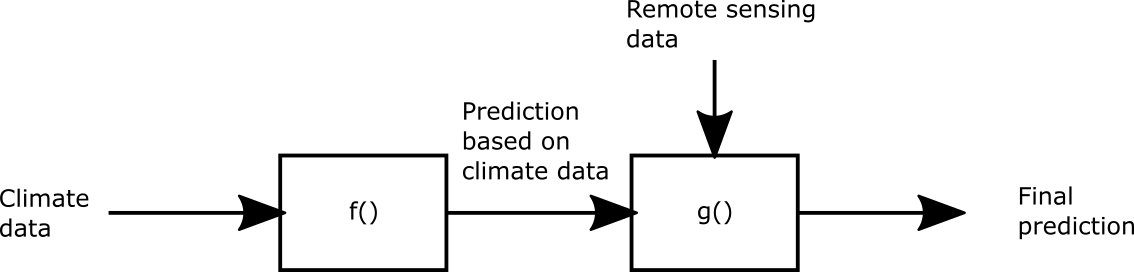
\includegraphics[scale=0.5]{VectorGraphics/HierarchicalClassification.png}
\caption{\label{fig:chClassificationTechniques:HierarchicalClassification}Visualization of the hierarchical model.}
\end{figure}

This hierarchical model has since been applied in combination with e.g.\ stacked SDMs \parencite{cord_remote_2014}. However, from a statistical point of view this approach is not well motivated. The main drawback of this approach is that interaction effects between the climate and remotely sensed variables cannot be taken into account. Furthermore, since there is usually quite some correlation between the climate and remotely sensed variables model selection is hampered. For example, if a remotely sensed variable is fundamental in determining the niche and highly correlated with a climate variable that is not as relevant for defining the niche the climate variable will usually end up in the model instead of the remotely sensed variable. Because of these drawbacks this approach will not be investigated.









\chapter{Reducing the number of explanatory variables}
\label{ch:ReducingTheNumberOfExplanatoryVariables}

\section{Introduction}
The explanatory variables used in SDMs are often correlated. Such high correlation can be an indication of redundant information in the data-set. Moreover, since there is usually no knowledge about which variables make up the niche of a species and irrelevant predictors might be included into the model. It is well known that this can lead to over-fitting and unstable predictions. In this chapter we describe some methods to deal with large sets of correlated predictors. More specifically, in Section \ref{sec:DimensionalityReduction} we introduce methods that transform the input space. In Section \ref{sec:Regularization} techniques that penalize ``large'' models are introduced. Finally, Section \ref{sec:SubsetSelectionMethods} deals with step-wise variable selection methods.

\todo[inline]{elaborate on problems when using models for prediction vs interpretable models, see Dorman et al. and Harel 2001 (see paper references Dorman)} 

For a review of methods to deal with correlated covariates in ecology we refer to \cite{dormann_collinearity:_2013}. Finally, these automatic selection procedures are of course not meant to replace a well founded motivation of why certain predictors should be selected. A discussion of how the available data, scale of the predictors, etc.\ should influence the decision of using a complex or a simple model can be found in \cite{merow_what_2014}.

\section{Dimensionality reduction}
\label{sec:DimensionalityReduction}
\todo[inline]{Discuss the effect of the number of background observations ?}
Dimensionality reduction techniques can be used to obtain a new, often lower-dimensional, representation of important structures in the input space. This can be particularly useful when two or more explanatory variables are proxies of one underlying latent variable. For example, there are multiple indices that indirectly measure the amount of vegetation. A combination of these indices might be a better indicator of the amount of vegetation than the individual indices. The dimensionality reduction techniques that are used in this thesis use only the input space and ignore the outcome values. It should however be noted that there are other dimensionality reduction techniques that do take into account the relationship between input and output variables, e.g.\ partial least squares \parencite[see e.g.][]{marx_iteratively_1996}.

\subsection{Principal component analysis}
Often principal component analysis (PCA) is introduced as a method which constructs uncorrelated linear combinations of the variables, these new variables are called principal components. However, for our purposes it might be more interesting to view PCA as a way to find a low dimensional affine subspace such that when the original data is projected onto this subspace the ``information loss'' is minimal. One possible characterization of PCA is that a set of $K$ orthonormal vectors $\bm{u}_i$ and an offset vector $\bm{b}$ are constructed so that
\[\sum_{i=1}^{N} \sum_{j=1}^{K} \vert \vert \bm{x}_i - \bm{x}_i'\bm{u}_i\bm{u}_i - \bm{b} \vert \vert_2^2 \]
is minimized. It can be shown that for a certain $K$ this sum is minimized when the $\bm{u}_i$ are the eigenvectors corresponding with the $K$ largest eigenvalues of the covariance matrix. A prototype scenario is shown in Figure \ref{fig:PCA}.\\

\begin{figure}[!htb]
\centering
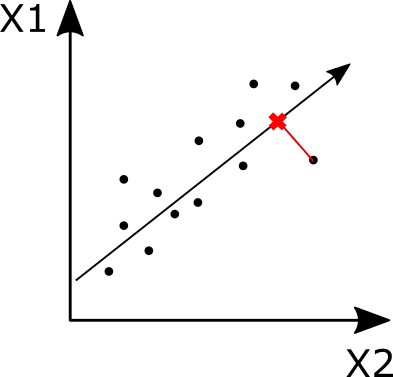
\includegraphics[scale=0.5]{VectorGraphics/PCA.png}
\caption{\label{fig:PCA}Visualization of the a typical scenario where PCA is useful.}
\end{figure} 


Once we have calculated the principal components they can be used as the explanatory variables in one of the models of Chapter \ref{ch:ClassificationTechniques}. Since the new variables are uncorrelated and some irrelevant noise in the predictors might be removed the resultant models often exhibit less variance. \\

There are multiple criteria based upon which the number of principal components, $K$, can be chosen. One possibility is to plot the so-called ``explained'' variance versus the number of components and look for either a kink or a point where a certain percentage of variance is explained. If PCA is combined with a classification method it is usually more appropriate to use cross-validation to select the number of principal components. We will use the cross-validation approach.\\

It should be clear that the main disadvantage of PCA is that it only allows for linear representations of the data. Hence, PCA will often be useless if the observations are scattered around a non-linear manifold. For example in Figure \ref{fig:PCACircle} there is a clear underlying space that is one dimensional. However, using the first principal component of this fictional data-set would lead to as big an ``information'' loss as using just one of the original axes. For the sake of completeness we mention that there are extensions of PCA that use non-linear manifolds instead of linear ones, e.g.\ principal curves and surfaces \parencite{hastie_principal_1989}. \\

\begin{figure}[!htb]
\centering
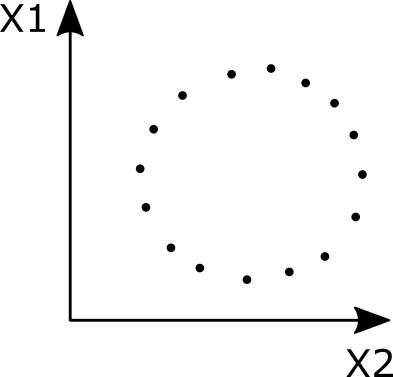
\includegraphics[scale=0.5]{VectorGraphics/PCACircle.png}
\caption{\label{fig:PCACircle}Visualization of the a scenario where PCA is useless.}
\end{figure}



\subsection{Kernel principal component analysis}
A popular and computationally efficient non-linear dimensionality reduction technique is kernel PCA \parencite{scholkopf_kernel_1997}. In kernel PCA the elements of the input space $\mathcal{X}$, in our case we have $\mathcal{X} = \mathbb{R}^p$, are mapped to a Hilbert space $F$. We will denote the map as: 
\[\bm{\phi}(\cdot): \mathcal{X} \to F.\]
In this new vector space a PCA is conducted and new coordinates are obtained. A visual presentation of these steps is given in Figure \ref{fig:KernelPCA}. \\
\begin{figure}[!htb]
\centering
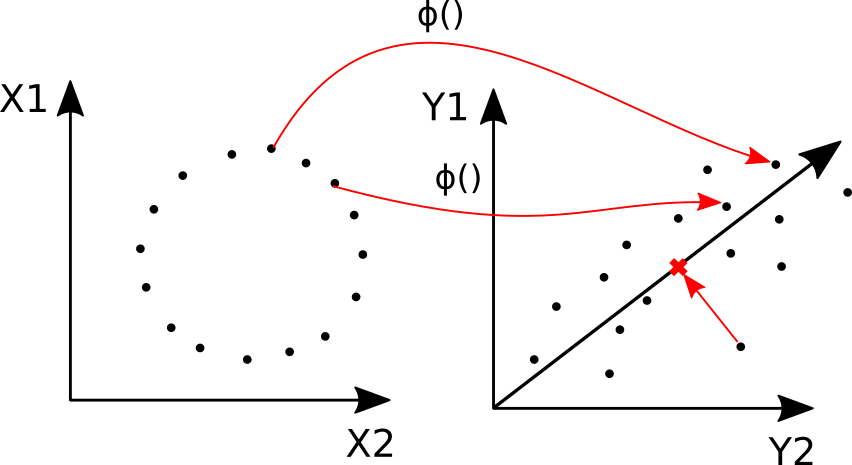
\includegraphics[scale=0.5]{VectorGraphics/KernelPCA.png}
\caption{\label{fig:KernelPCA}Visualization of kernel PCA.}
\end{figure}

One attractive property of kernel PCA is that we do not need to actually compute $\phi(\bm{x})$. More specifically we only need to compute the so-called kernel matrix $\mathbb{K}$
\[\mathbb{K}_{ij} = \langle \bm{\phi} (\bm{x}_i), \bm{\phi} (\bm{x}_j)  \rangle = k(\bm{x}_i,\bm{x}_j).\]
In general it can be shown that, under some regularity conditions, for any kernel function
\[k(\cdot,\cdot): \mathcal{X} \times \mathcal{X} \to \mathcal{R}\] 
there exists a corresponding $\bm{\phi}(\cdot)$ and Hilbert space $F$. Hence usually one specifies the kernel function instead of the map $\phi(\cdot)$.\\ 

Popular choices of the kernel function include:
\begin{itemize}
\item The polynomial kernel $k(\bm{x},\bm{y}) = (\bm{x}' \bm{y} + c)^d$.
\item The radial basis kernel (RBF kernel) $k(\bm{x},\bm{y}) = \exp{(-\frac{\vert \vert \bm{x} -\bm{y}\vert \vert ^2}{\sigma})}$, with $\sigma > 0$. 
\item The hyperbolic tangent kernel, $k(\bm{x},\bm{y}) = \tanh{(\sigma \bm{x}^t \bm{y} + c)}$.
\end{itemize}
In these representations the $\sigma$, resp.\ $c$, parameter can be seen as a scale, resp.\ offset, parameter. The value of these parameters is in general selected by using cross validation. We will focus on the RBF kernel, this kernel is usually used when no prior information is available \parencite{JSSv011i09}.  \\

A disadvantage of kernel PCA is that it is not always clear which kernel should be used. For our goals, combining kernel PCA and a classification method, we can use cross-validation and treat the type of kernel as a tuning parameter. Furthermore, it is not always particularly clear what the new features are supposed to represent (we might not even know in which Hilbert space we are working). An R implementation of kernel pca is provided as part of the \textsc{kernlab} package \parencite{JSSv011i09}.

\subsection{Presence versus background data}
\label{sec:dimRedPrVSBG}


\section{Regularization}
\label{sec:Regularization}
When one uses regression methods, e.g. logistic regression or ANNs, in combination with a large set of correlated predictors the obtained coefficients are often excessively large and unstable. To combat this large coefficients can be penalized such that the solution consists of shrunken coefficients. To do this the standard minimization problem
\[\widehat{\bm{\gamma}} = \argmin_{\bm{\gamma}} L(\bm{y},\bm{\gamma})\]
is adjusted to \[\widehat{\bm{\gamma}} = \argmin_{\bm{\gamma}} L(\bm{y},\bm{\gamma}) + J(\bm{\gamma},\bm{\lambda}).\]
In this representation the function $ J(\bm{\gamma},\bm{\lambda})$ is usually a monotonically increasing function in $\bm{\gamma}$. Furthermore, the $\bm{\lambda}$ parameters are used to control ``the amount of regularization'' and are often selected by using cross-validation. Finally, the described regularization methods can be used in conjunction with logistic regression by using the \textsc{glmnet} \parencite{glmnet} package.

\label{sec:Regularization}
\subsection{Ridge regression / $L_2$ regularization}
\label{sec:L2Regularization}
Ridge regression (also called $L_2$ regularization) is obtained when the Euclidean norm of the coefficients is used as the penalization function:
\[J(\bm{\gamma},\lambda) = \lambda \vert \vert \bm{\gamma} \vert \vert ^2 _2.\]
We immediately see that small $\lambda$'s correspond to a small amount of regularization and the non-penalized solution is obtained when $\lambda = 0.$ Furthermore, when $\lambda >>$ the coefficients are shrunken to zero. A typical evolution of the coefficients in function of the regularization parameter can be found in Figure \ref{fig:RidgeTrace}.\\ 

\begin{figure}[!htb]
\centering
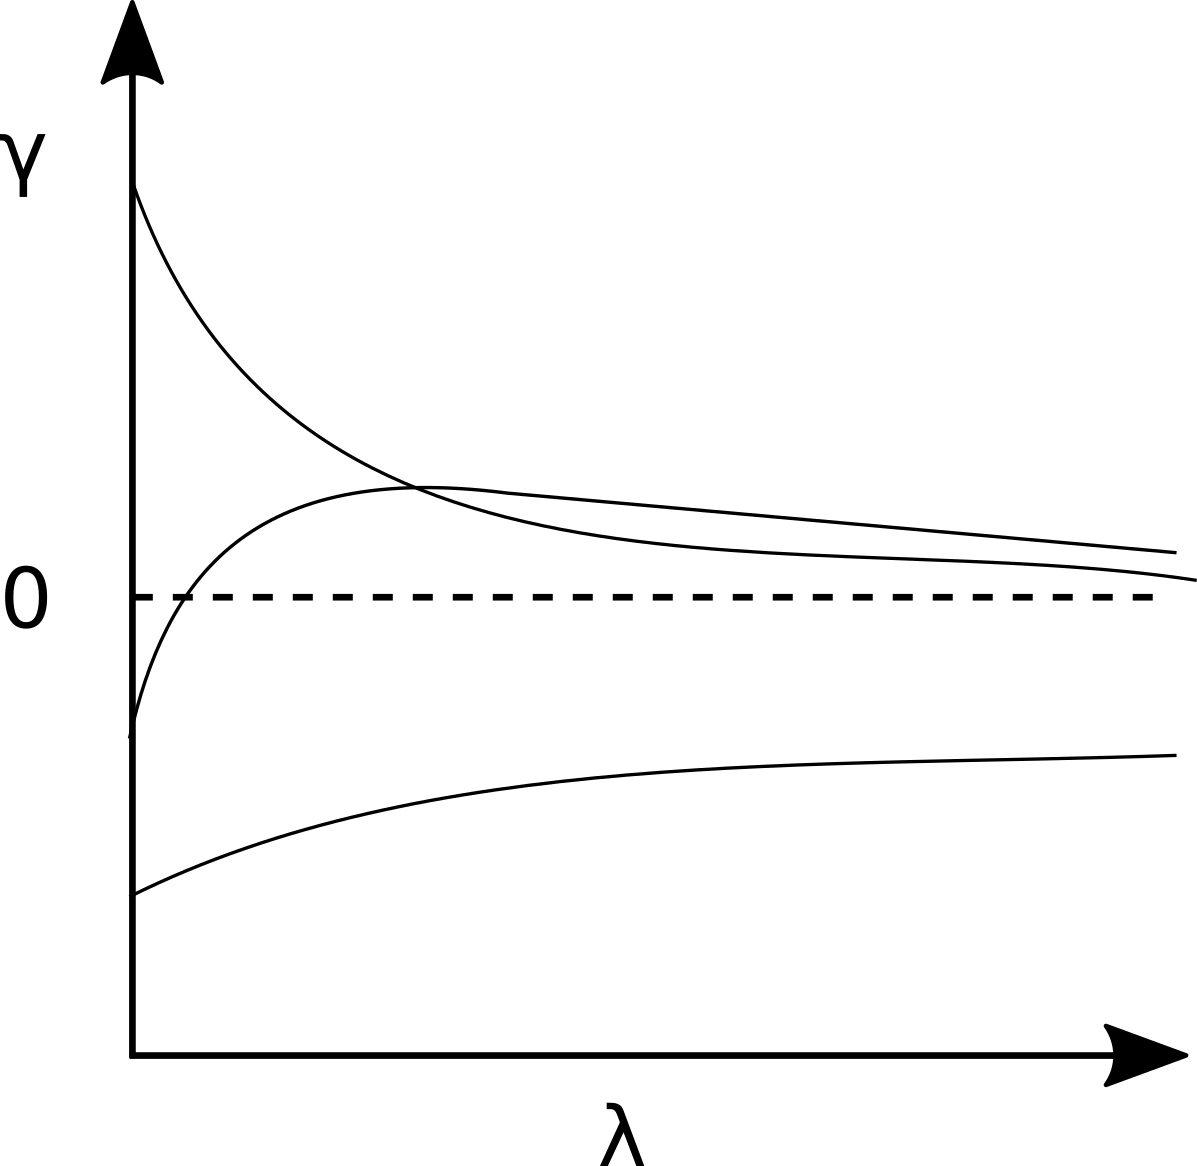
\includegraphics[scale=0.75]{VectorGraphics/ridgeTrace.png}
\caption{\label{fig:RidgeTrace}A stereotypical evolution of the regression parameters in combination with the ridge parameter.}
\end{figure}

It is clear that rescaling the covariates will usually lead to different penalized coefficients. It is therefore recommended to standardize the covariates before applying ridge regression.\\

Advantages of using an $L_2$ penalty include:
\begin{itemize}
\item The penalty is differentiable and hence compatible with e.g.\ backpropagation.
\item For most regression problems it is easy to adopt the standard algorithms to include the $L_2$ penalty.
\item It is usually no problem if the number of variables is larger than the number of observations.
\end{itemize}
The biggest disadvantages is that all the predictors are kept in the model, i.e.\ usually no coefficients are equal to zero. \\

Finally, we note that $L_2$ regularization is also called weight decay when it is used in combination with neural networks. 

\subsection{Lasso / $L_1$ regularization}
\label{sec:Lasso}
Another popular option was proposed by \cite{tibshirani_regression_1996}. He suggested to use the absolute norm (also called the $L_1$ norm or Manhattan distance) as penalty function, or thus the minimization problem becomes: \[J(\bm{\gamma},\bm{\lambda}) = \lambda \vert \vert \bm{\gamma} \vert \vert _1 = \lambda \sum_{i=1}^p \vert \gamma_j \vert.\]
The $L_1$ penalty term is also called the least absolute shrinkage and selection operator (lasso). Unlike $L_2$ regularization, the lasso solution will usually contain some coefficients that are equal to zero. This implies that, in addition to the parameter shrinkage, the lasso performs some form of automatic variable selection. A typical parameter trace can be found in Figure \ref{fig:LassoTrace}. \\
\begin{figure}[!htb]
\centering
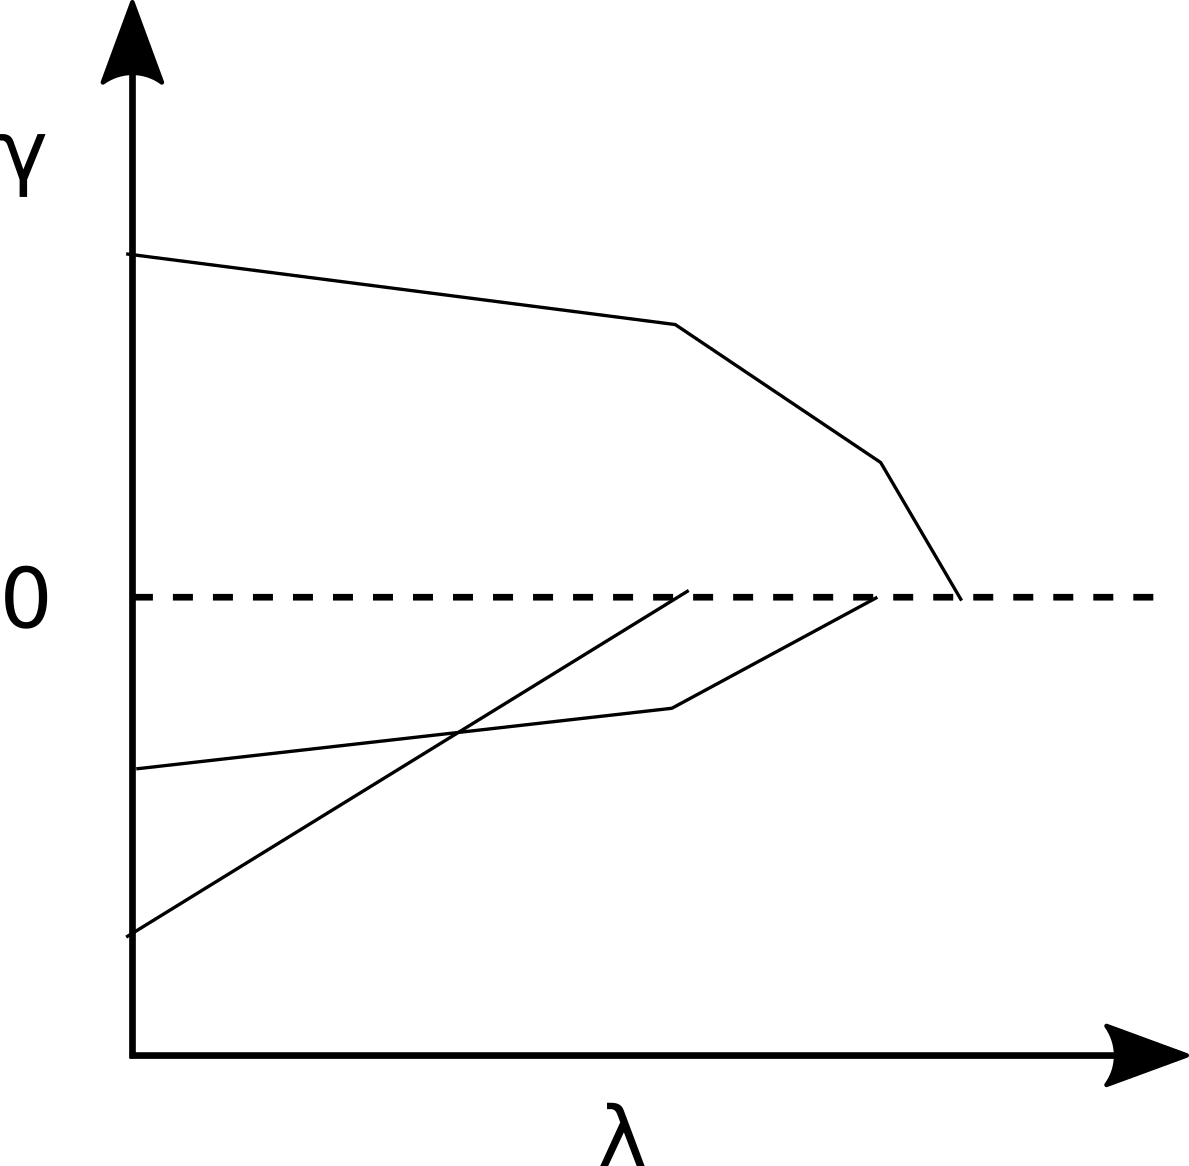
\includegraphics[scale=0.75]{VectorGraphics/lassoTrace.png}
\caption{\label{fig:LassoTrace}Visualization of the typical evolution of the regression parameters in combination with the lasso parameter.}
\end{figure}

Usually the shrinkage parameter is selected by using cross-validation. The main advantage is that the lasso performs both shrinkage and parameter selection at once. Disadvantages include:
\begin{itemize}
\item The lasso penalty is not differentiable and hence one cannot use algorithms like backpropagation.
\item At most $n$ variables are included in the model.
\item If there is a group of highly correlated variables usually only one will be selected. Sometimes the variable that is selected is rather arbitrary.
\end{itemize}

\section{Subset selection methods}
\label{sec:SubsetSelectionMethods}
Subset selection methods are a set of older methods to reduce the number of explanatory variables. Although subset selection methods are often criticised for ignoring problems with bias, multiple testing, etc. \parencite{whittingham_why_2006} they are still popular. In this section three different subset selection techniques are discussed. \\

\subsection{Best subset selection}
The most elementary technique in this set of methods is best-subset selection. Best subset selection consists of fitting a model for each combination of predictors and then selecting the best model from these. What constitutes the best model depends on the goals of the study but often used selection criteria include: AIC, missclassifcation error, p-values, etc. The biggest limitation of best-subset selection is that when the number of predictors increases there is an exponential increase in computational complexity. In particular, if there are $p$ potential terms to be included we need to fit $2^p$ models. Since we have $33$ variables this method is infeasible for our purposes.\\

\subsection{Stepwise subset selection}
A second subset selection method is backward-stepwise selection. This method starts with the model containing all $p$ predictors. In the second step of the algorithm we try removing each predictor from the full model and select the most optimal model from the models with $p-1$ covariates. In the third step we remove each predictor from the model obtained in the second step, fit a model with $p-2$ predictors, and select the best model from these. This process is repeated until there is no improvement possible. One of the most important disadvantages of this method is that it is quite variable. Furthermore, for some algorithms (e.g.\ logistic regression) we need to have $p < n$.
\\

Forward-stepwise selection is basically the reverse of the backward-stepwsie method. More particuarly, one starts with the model containing only an intercept. The the variable that leads to the largest improvement is added. And this process is repeated until the performance criterion can not be improved any further. The main advantage of this method over backward-stepwise selection is that it is generally less variable. On the other hand, this method usually leads to a bigger bias. Another limitation of forward-stepwise subset selection is that it fails if, in order to minimize some selection criterion, two predictors need to be included at the same time.\\

\subsection{Univariate pre-screening}
\subsubsection{Underlying idea}
Univariate pre-screening is somewhat related to forward-stepwise regression. Just as in forwar-stepwise selection we start by fitting the $p$ models including an intercept and one predictor. In the second step a final model is fitted by using all predictors for which the corresponding model from the first step met a certain criteria, e.g. a significant p-value. \\

An advantage of this method is that, compared to the other subset selection methods that were discussed, it is computationally efficient. 
An important disadvantage of univariate pre-screening is that, because of its univariate nature, the correlation between predictors is ignored. Hence, highly correlated predictors will often be included in the final model. It is interesting to note that the multiple testing problem is particularly clear when using this method. However, since we know the exact number of tests it is quite easy to control some multiple testing error rate instead of the type 1 error. Since we will not use standard univariate pre-screening we will not discuss methods to control the multiple error rate. For two methods to control a multiple testing error rate we refer the interested reader to e.g.\ \cite{holm_simple_1979} or \cite{benjamini_controlling_1995}.

\subsubsection{Taking the correlation into account}
In ecological research a variation on univariate pre-screening that tries to take into account the correlation is regularly used, e.g.\ \cite{cord_remote_2014}. The method, which we will call select07, selects one variable from each set of highly correlated variables. The algorithm works as follows:
\begin{enumerate}
\item Make a set $A$ of all variables.
\item Calculate all correlations.
\item For each pair of variables with $|r| > 0.7$ we fit a univariate model.
\item For each pair selected in step 3. we remove the worst\footnote{As usual, different performance measures can be used, e.g. AIC, p-values, etc.} performing variable from $A$.
\item Fit a final model that includes all variables left in the set $A$.
\end{enumerate}
An implementation of this method was provided by \cite{dormann_collinearity:_2013}. In this implementation both GAMs and logistic regression can be used and the performance of the univariate models is measured by the AIC value. Finally we note that using $|r| > 0.7$ is quite arbitrary, however this threshold seems quite popular in SDM.

\section{Taking the scale hierarchy into account}
\label{sec:TakingTheScaleHierarchyIntoAccount}
\todo[inline]{double check which kind of models / residuals the used in the paper}
\cite{thuiller_we_2004} used a hierarchical model selection approach. More specifically, they investigated the effect of adding land-cover data to models build with climate data. To do this they used the following three steps:
\begin{enumerate}
\item A model with only climate variables is constructed by using a stepwise selection method.
\item Regress the residuals of the climate model on the land-cover variables and use a stepwise selection method to select the most influential variables.
\item Build a new model with the selected climate and land-cover variables.
\end{enumerate}
Although the focus in the article was on stepwise regression techniques, the same procedure can be applied in combination with other variable selection methods. However, this hierarchical approach has a clear disadvantage, it cannot consider interactions between climate and land-cover variables. Furthermore, the obtained solution will most often be sub-optimal compared to using a selection procedure with all the variables. Hence we see little reason to consider this approach any further.


\section{Meaningful combinations of classification and }
\label{sec:combinations}
 

For each method of Chapter \ref{ch:ClassificationTechniques} a ``vanilla'' model will be considered. The vanilla logistic regression and ANN model use all predictors except the agriculture land cover class and BIO7. These two predictors are removed to avoid computational problems associated with design matrices that are not of full rank. For the vanilla GAM all predictors are used together with GCV to select the smoothness parameters. The vanilla MaxEnt model is the standard MaxEnt model with the default parameters \parencite{phillips_modeling_2008}. Finally, the vanilla version of boosted regression trees is just the standard implementation. \\

Next to the vanilla models ten combinations of classification algorithms and methods to reduce the number of variables will be considered, see Table \ref{table:combinations}. Combinations that are not included were often not computationally feasible to implement, e.g.\ combing kernel PCA and GAMs, or not meaningful, e.g.\ $L_1$ regularization combined with boosted regression trees. Furthermore, following the remarks in Section \ref{sec:dimRedPrVSBG} when PCA or kernel PCA are used in combination with presence-only data three different version will be considered: \begin{enumerate}
\item a version where the PCA is performed on the predictor values associated with background and presence locations.
\item a version where the PCA is performed only on the predictors values associated with background locations.
\item a version where the PCA is performed only on the predictors values associated with presence locations.
\end{enumerate}
In total $20$ methods are used when presence-only data is considered and $14$ when presence-absence data is considered.


\begin{table}[!htb]
\makebox[\textwidth][c]{
\begin{tabular}{l@{\hskip 1cm}cccccccc}
\toprule
 								& PCA				& kernel PCA			& $L_2$ penalty	& $L_1$ penalty & stepwise selection & select07 \\
\midrule
 								\\
Logistic regression 			& \ding{51}			& \ding{51}			  	& \ding{51}			 	& \ding{51} & \ding{51}& \ding{51}\\ 
Additive logistic regression 	&			&			  	& \ \ding{51}\tablefootnote{Regularization of the ``wiggliness'' instead of the coefficients, see Section \ref{sec:GAM}} 		&  & & \ding{51}
\\
Artificial neural networks 		&			&				& \ding{51}	\\
Boosted regression trees 		& 	\\
MaxEnt							& 			& 						&						& \ding{51} \tablefootnote{Using five fold CV to select the $L_1$ regularization parameter instead of using the default parameter.} \\
\bottomrule
\end{tabular}}
\caption{\label{table:combinations}Table with the combinations of classification and dimensionality reduction techniques that are considered.}
\end{table}

\chapter{Applications}
\label{ch:Applications}
\section{Introduction}
The use of the area under the receiver operating curve (AUC) as a measure of performance in SDM is discussed in Section \ref{sec:AUC}. In Section \ref{sec:POData} (resp.\ \ref{sec:PAData}) the performance of the techniques is discussed in the case of presence-only (resp.\ presence-absence) data. In both these sections the models were fit by using a training set and then the AUC values were calculated on a test set. The training set consists of \nicefrac{3}{4}'th of the data while the test set contains the other \nicefrac{1}{4}'th.\\


\section{AUC as a measure of classification performance in SDM}
\label{sec:AUC}
To measure the performance of the classification method the AUC is used. Using the AUC to measure the performance of SDMs has been criticized \parencite{lobo_auc:_2008, jimenez-valverde_insights_2012}. However, most of the issues that are usually raised are not of particular interest in our case. Before studying the AUC values it is interesting to note that there are three main sources of randomness in the calculation of the mean AUC values across the different species. \\ 

First of all, in our set-up we could consider the species that are considered as drawn from a pool of all species in the databases. Of course this assumption is violated since we selected the species conditional on certain characteristics. Hence a more accurate depiction would be to say that the species are a stratified sample from the pool of available species.  \\

Secondly, the parameters in the classifications methods are estimated by using the training set. The elements of the training set can be seen sample of presence, and background or absence points from the corresponding distributions. The predicted probabilities, and the AUC, are therefore also dependent on the sample of points used.\\

Thirdly, the AUC is calculated on the test set which again consists of a sample of random presence, and background or absence points from the corresponding distributions. Thus even if the classifier was fixed we would get different AUC values if we use different test sets. \\

It is well known that the AUC statistic is equivalent to the Mann-Whitney U test statistic \parencite{hanley_meaning_1982}. Therefore the theory surrounding the Mann-Whitney U test statistic can provide us with standard errors (SE), asymptotic distributions, etc. However, these results were derived by assuming that the classifier is fixed. Given that also the training set and the considered species can be seen as a random sample these results are not directly applicable. A rigorous way to inspect the distribution of the AUC values would be to use a bootstrap method to construct e.g.\ confidence intervals. In our situation this is, however, computationally infeasible. In the end we opted to only report standard deviations (SD) and mean values.\\

\section{Presence-only data}
\label{sec:POData}
\subsection{Results}
All the methods described in Chapter \ref{ch:Implementations} were fitted on the GBIF data. A plot of the AUC values can be found in Figure \ref{fig:PrOnlyAUC} and summary measures can be found in Table \ref{tab:PrOnlyAUC}. Few rigorous tests are performed in this section. This because, given the small sample size and the fact that the AUC values are quite close, the power of such tests, using the usual $5\%$ significance level, is very low. Therefore the discussion of the results is rather short and mainly used as a preliminary study to generate interesting research questions for the simulation study of Chapter \ref{chap:SimulationStudy}. \\


\begin{table}[!htb]
\makebox[\textwidth][c]{
\begin{tabular}{lcccccc}
 & \multicolumn{2}{c}{All variables} & \multicolumn{2}{c}{Bioclimatic variables} & \multicolumn{2}{c}{Difference}\\
\cline{2-3} \cline{4-5} \cline{6-7}\\
Method & Mean AUC & SD & Mean AUC & SD & Mean AUC & SD \\
\midrule
Logistic: vanilla               & 0.934 & 0.045 & 0.916 & 0.070 & 0.019    & 0.053 \\
Logistic: backward              & 0.772 & 0.266 & 0.934 & 0.035 & -0.162   & 0.262 \\
Logistic: forward               & 0.661 & 0.242 & 0.599 & 0.277 & 0.062    & 0.330 \\
Logistic: PCA                   & 0.891 & 0.077 & 0.881 & 0.087 & 0.010    & 0.070 \\
Logistic: presence PCA          & 0.838 & 0.172 & 0.887 & 0.090 & -0.049   & 0.101 \\
Logistic: background PCA        & 0.893 & 0.079 & 0.890 & 0.077 & 0.003    & 0.054 \\
Logistic: kernel PCA            & 0.933 & 0.050 & 0.922 & 0.058 & 0.011    & 0.030 \\
Logistic: presence kernel PCA   & 0.947 & 0.033 & 0.927 & 0.052 & 0.020    & 0.040 \\
Logistic: background kernel PCA & 0.937 & 0.048 & 0.935 & 0.039 & 0.002    & 0.028 \\
Logistic: lasso                 & 0.938 & 0.041 & 0.924 & 0.057 & 0.014    & 0.037 \\
Logistic: ridge                 & 0.930 & 0.047 & 0.908 & 0.063 & 0.022    & 0.039 \\
Logistic: select07              & 0.938 & 0.040 & 0.915 & 0.058 & 0.023    & 0.032 \\
GAM: auto selection             & 0.928 & 0.072 & 0.935 & 0.033 & -0.008   & 0.069 \\
GAM: vanilla                    & 0.912 & 0.086 & 0.936 & 0.038 & -0.024   & 0.090 \\
GAM: select07                   & 0.940 & 0.050 & 0.938 & 0.036 & 0.002    & 0.039 \\
MaxEnt                          & 0.921 & 0.055 & 0.932 & 0.041 & -0.011   & 0.028 \\
MaxEnt Vanilla                  & 0.899 & 0.099 & 0.919 & 0.049 & -0.020   & 0.076 \\
ANN                             & 0.946 & 0.046 & 0.948 & 0.032 & -0.003   & 0.040 \\
ANN: vanilla                    & 0.926 & 0.058 & 0.934 & 0.039 & -0.008   & 0.048 \\
GBM                             & 0.958 & 0.032 & 0.944 & 0.033 & 0.014    & 0.030 \\
\bottomrule
\end{tabular}}
\caption{\label{tab:PrOnlyAUC}Summary of the AUC values of the different classifiers fitted on the presence-only data.}
\end{table}

\begin{figure}[!htb]
\center
\makebox[\textwidth][c]{%
	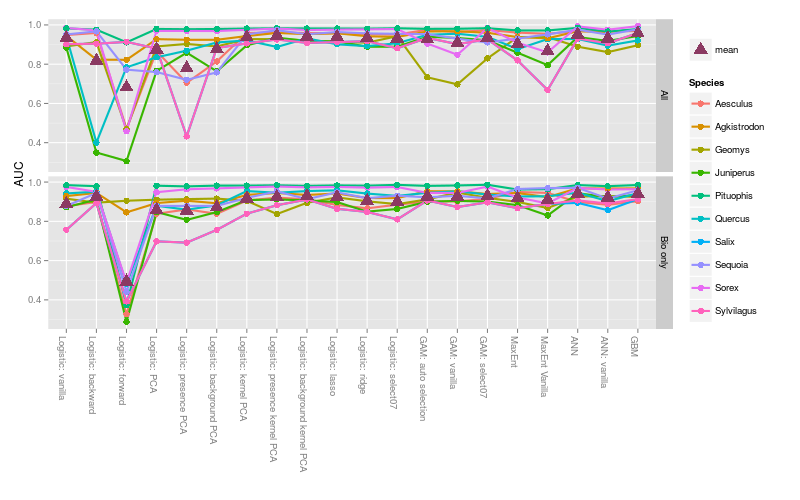
\includegraphics[scale=0.70]{Plots/AUCPlot.png}
}
\caption{\label{fig:PrOnlyAUC}AUC values of the different classifiers fitted on the presence-only data.}
\end{figure}


First of all, it is interesting to note that logistic regression performs quite well. There is a small, non-significant, decrease in mean AUC value when only the bioclimatic variables are considered.\\

The two stepwise selection methods have relatively small mean AUC values and large SDs when all variables are considered. The high SDs indicate that these methods are inherently variable and hence usually lead to unstable predictions. When only the bioclimatic variables are considered the same is true for the forward stepwise selection method, on the other hand backward stepwise selection performs quite well. This could be explained by the fact that the backward selection method becomes a lot more variable when variables with little explanatory power are added. Finally, in comparison with the vanilla logistic regression method the stepwise methods perform quite badly. However, since in the vanilla logistic method only first order terms are considered it might be unfair to say that stepwise selection is inherently worse and a comparison with a logistic regression model with the same polynomial expansion might have been more appropriate. \\ 


The MaxEnt implementation with the default settings performs worse than the implementation in which the penalization parameter is selected by CV. Although MaxEnt is very popular in SDM applications it does not seem to perform better than simpler models as logistic regression. Even though our small sample size does not allow us to dispute the popularity of MaxEnt our results seem to show that even if there is a gain in performance over e.g.\ logistic regression it is likely quite small and one might wonder if the loss of interpretability and increased computational cost is worth a small gain in performance. Furthermore, it seems that in most applications of SDM the default value of the penalization parameter is used while our results seem to show that using CV leads to some improvements. \\

GBMs and ANNs seem to consistently lead to high AUC values with low standard deviations. Although these methods are sometimes used in practice they are far less popular than the MaxEnt method. Given our results it seems like MaxEnt might be overused and it seems appropriate to at least consider some other machine learning methods when building SDM. \\ 

None of the PCA logistic regression methods seem to perform well, i.e.\ the mean AUC is lower than the mean AUC of logistic regression and the SDs are quite large. Both when only the bioclimatic variables and when all variables are used at least one of the KPCA logistic regression methods tends to outperform the logistic regression model. At first glance there does not seem to be a systematic difference between using the presence or the background observations in the (K)PCA methods. To rigorously test this two Wilcoxon signed-rank tests were performed. The p-value corresponding with the test for the PCA (resp.\ KPCA) method is $0.32$ (resp.\ $0.11$) and hence the null-hypothesis of no difference between the methods is accepted. \\

The three version of GAMs that we consider all seem to perform better than logistic regression when only the bioclimatic variables are considered. When all variables are considered the select07 variable selection method in combination with a GAM still performs decently while the two other methods seem to deteriorate slightly.  \\

The penalized logistic regression models perform approximately on par with the standard logistic regression model. Finally, the logistic regression model combined with the select07 rule seems to slightly outperform the standard logistic regression model when bioclimatic variables are considered and on par when all variables are used. \\

To test whether or not using only the bioclimatic variables has a profound effect a Wilcoxon signed-rank test was performed for each method. These tests are of interest because on one hand they provide information on the usefulness of non-bioclimatic variables, i.e. is there an increase in classification performance. Also a decrease of the AUC values is of interest, it could namely be interpreted as adding irrelevant predictors which lead to over-fitting. Even before performing a multiple testing correction none of the tests were significant at the $5$\% level. It is therefore concluded that in this limited study there is no statistically significant difference between using only the bioclimatic variables or all variables. 

\section{Presence-absence data}
\label{sec:PAData}
In this section the classification methods are used in combination with the FIA presence-absence data. First of all, although a variation of the MaxEnt method can be used for presence-absence data this is nearly never done. Furthermore, instead of fitting three different variations of (K)PCA logistic regression it was decided to only use the standard approach. This was done to speed up the computations, and unlike in the presence-only scenario the absence points are ``real'' observations. Since only five species were considered there are no statistically significant results in this section. The inspection is mainly done to make sure that the different methods show approximately the same performance characteristics for both presence-only and presence-absence data. The results can be found in Section \ref{sec:PAResults}. Finally, because there are at between $42029$ and $287860$ plot locations available the fitting of the models leads to computational problems. A solution to these problems is proposed in Section \ref{sec:CaseControlSubsampling}.
\subsection{Case-control sampling}
\label{sec:CaseControlSubsampling}
Because of computational considerations it was decided to use a subset of the presence-absence data to fit the models upon. More particularly, the subsample consists of all the presence points and $5000$ randomly sampled absence points. This is a form of case-control sampling and the effect of doing this has been studied \parencite{king_logistic_2001}. \\

In the case of logistic regression some algebra along the lines of Equation \ref{eq:IPPSampling} shows that only the intercept is affected by the sub-sampling \parencite{king_logistic_2001}. Although the underlying coefficients stay the same the variance of the estimators increases slightly. Because we only subsample the absence points this increase should be somewhat limited. Intuitively it makes sense that a rare presence point contains more information about the coefficients than one of the abundant absence points. In the case of logistic regression this can rigorously be deduced by observing that a term of the form $P(Y=1|\bm{X} = \bm{x}) \left[1- P(Y=1|\bm{X} = \bm{x}) \right]$ turns up in the variance expression. Usually this term is quite a lot smaller for the abundant cases and hence leaving some out does not lead to a huge increase of the variance. \\ 

Although the previous paragraph focusses on logistic regression the same reasoning can be applied to the other methods considered. Finally, in the last two decades there has been quite some research on issues related to imbalanced data-sets and perhaps more efficient ways of dealing with the imbalance exist, see e.g.\ \cite{chawla2005data} for an overview of other methods. \\

\subsection{results}
\label{sec:PAResults}
The mean and and the standard deviations can be found in Table \ref{tab:PrAbAUC} and Figure \ref{fig:PrAbAUC} shows a plot of the estimated AUC values. \\

\begin{table}[!htb]
\makebox[\textwidth][c]{
\begin{tabular}{lcccccc}
 & \multicolumn{2}{c}{All variables} & \multicolumn{2}{c}{Bioclimatic variables} & \multicolumn{2}{c}{Difference}\\
\cline{2-3} \cline{4-5} \cline{6-7}\\
Method & Mean AUC & SD & Mean AUC & SD & Mean AUC & SD \\
\midrule
Logistic: vanilla    & 0.961 & 0.027 & 0.951 & 0.041 & 0.010   & 0.022 \\
Logistic: backward   & 0.682 & 0.301 & 0.703 & 0.276 & -0.021  & 0.355 \\
Logistic: forward    & 0.774 & 0.284 & 0.660 & 0.333 & 0.115   & 0.208 \\
Logistic: PCA        & 0.913 & 0.084 & 0.926 & 0.063 & -0.013  & 0.055 \\
Logistic: kernel PCA & 0.950 & 0.052 & 0.922 & 0.086 & 0.028   & 0.041 \\
Logistic: lasso      & 0.960 & 0.042 & 0.968 & 0.022 & -0.008  & 0.025 \\
Logistic: ridge      & 0.957 & 0.044 & 0.948 & 0.049 & 0.009   & 0.016 \\
Logistic: select07   & 0.756 & 0.239 & 0.859 & 0.206 & -0.102  & 0.219 \\
GAM: auto selection  & 0.925 & 0.098 & 0.954 & 0.038 & -0.029  & 0.062 \\
GAM: vanilla         & 0.877 & 0.117 & 0.927 & 0.074 & -0.049  & 0.098 \\
GAM: select07        & 0.948 & 0.062 & 0.954 & 0.052 & -0.006  & 0.019 \\
ANN                  & 0.973 & 0.020 & 0.971 & 0.024 & 0.002   & 0.007 \\
ANN: vanilla         & 0.962 & 0.036 & 0.963 & 0.035 & -0.001  & 0.009 \\
GBM                  & 0.977 & 0.014 & 0.961 & 0.030 & 0.016   & 0.023 \\
\bottomrule
\end{tabular}}
\caption{\label{tab:PrAbAUC}Summary of the AUC values of the different classifiers fitted on the presence-absence data.}
\end{table}


\begin{figure}[!htb]
\center
\makebox[\textwidth][c]{%
	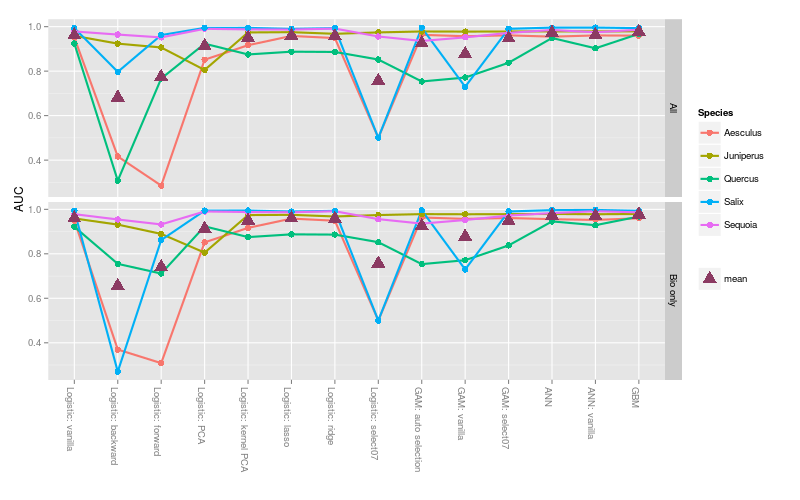
\includegraphics[scale=0.70]{Plots/AUCPAPlot.png}
}
\caption{\label{fig:PrAbAUC}AUC values of the different classifiers fitted on the presence-absence data.}
\end{figure}

It is readily seen that the logistic regression model performs quite well, i.e. it leads to relatively high average AUC values and its SD is quite low. The stepwise methods both have large SD and have the lowest average AUC values. The GBM and ANN methods are the two methods with the largest average AUC and both have relatively small SD. Unlike in the presence-only scenario the logistic07 methods has quite a large variance and performs quite badly. Finally, the differences between using the bioclimatic or all variables are extremely small, 



\section{Discussion}



\chapter{Simulation study}
\label{chap:SimulationStudy}

\section{Introduction}
In order to study the methods in more depth a simulation study will be done. The main advantage of this simulation study over using data on real species is that the variables that make up the species distribution can be decided upon. Because of the usual non-linear shape of the response-functions, the sampling design, \dots it is quite hard to set up a simulation study. Luckily the
\textsc{virtualspecies} package \parencite{virtualspecies, leroy2015virtualspecies} provides a simulation framework that allows the simulation of realistic species distributions. \\

\section{Overview of the \textsc{virtualspecies} package and the simulation set-up}
In order to justify using the samples generated by the \textsc{virtualspecies} package the internal process is quickly sketched. \\

First of all, the \textsc{virtualspecies} package generates a suitability raster, i.e.\ a raster containing high values for suitable habitat and vice versa, based upon a set of provided rasters of environmental variables. Since the package imposes no restrictions on the function that generates the values associated with the presence locations suitability from the provided variables, the suitability raster has to be converted into a probability of occurrence map. This can be done by using e.g.\ the logit function to map $\mathbb{R} \to [0,1]$. Once a raster containing the occurrence probability map is obtained a raster containing ones where the simulated species is present and zeroes otherwise can be obtained. This is done by sampling cells with a probability proportional to the probability of the occurrence and setting the cell value to $1$. From this raster a presence-only sample can be obtained by drawing random points within the cells that have a value of $1$.\\

It is interesting to note that the suitability raster is based upon the principal components of the variables over the whole study extent. Hence in our simulation study it is in some sense more appropriate to perform the (K)PCA logistic regression on the background points. \\

To facilitate the computations it was decided to select one area in which several random species are generated. In order to make sure that the environmental conditions can fluctuate within the distribution of one generated species to the next it was required that the selected area has to contain different types of habitat types. The obvious choice would be to use the contiguous United States, this is, however, computationally demanding. In the end it was decided to perform the simulation study on data contained within a rectangle that approximately corresponds to Washington state, see Figure \ref{fig:WashState}. Washington state has a big precipitation and temperature gradient because of the rain shadow created by the Cascade Range. This is also reflected in the fact that the types of habitat within this extent range from temperate rainforests, e.g.\ the Hoh Rainforest, to steppe- and dessert-like areas in Southeastern Washington.

\begin{figure}[!htb]
\center
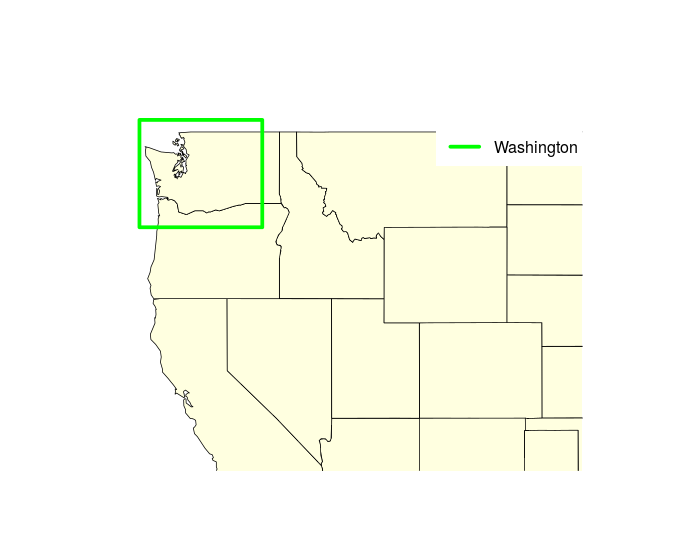
\includegraphics[scale=0.5]{Plots/WashingtonPlot.png}
\caption{\label{fig:WashState}Extent considered in the simulation study.}
\end{figure}

In order to study the generalizability of the methods it was decided that $5$ different species would be simulated. Furthermore, to be able to investigate the sample to sample variability of each method $5$ different presence-only samples were drawn for each simulated species. Since the mean (resp.\ median) number of observations of the presence-only datasets is $320.3$ (resp.\ $133.5$) it was decided to simulate $200$ occurrence points for each simulated dataset. \\

In Section \ref{sec:AUC} the various sources of the variability in the AUC values were discussed. Given that the interest is mainly in the training sample to training sample variability, it was decided to try to restrict the test sample to test sample variability to some extent. This can be done by taking a large test set. Using a sample of $1000$ occurrence and $1000$ background locations the standard error of the AUC value, conditional on the classifier, is $\approx 0.013$. This should be large enough to prevent the scenario where the test sample to test sample variability is much larger than the training to training sample variability.

\section{Model and estimators}
\label{sec:Estimators}
In order to be able to perform statistical inference an underlying model has to be proposed and estimators will be proposed. First of all the generated AUC values will be denoted by $Y_{ij}$ with $i \in \{1,\ldots,5\}$ indicating the species and $j \in \{1,\ldots,5\}$ indicates which sample of the $i$'th virtual species is considered. We assume that there is an underlying average AUC value $\mu$, for each sampled species there is then a species specific average AUC that deviates from $\mu$ by an amount equal to $\delta_i$ with $E(\delta_i) = 0$. Finally, because of training and test sample variability the estimated AUC will deviate from $\mu + \delta_i$ by an error $\epsilon_{ij}$ with $E(\epsilon_{ij}) = 0$. Hence:

\begin{equation}
\label{eq:SimModel}
Y_{ij} = \mu + \delta_i + \epsilon_{ij}.
\end{equation}

It is logically to assume that not only the $\delta_i$ and $\epsilon_{ij}$ are random but also that the $\text{Var}(\epsilon_ij) = \sigma_i^2$ is a species specific variance that is different for each species. For each method we are interested is in estimating:
\begin{itemize}
\item The mean $\mu$.
\item The expected variation of a classifier ``independent'' of the selected species or hence $E(\sigma^2) \equiv \tau^2$.
\item The difference between using all variables or only the bioclimatic variables, i.e. $\mu_{all} - \mu_{bio}$.
\end{itemize} 
It could be argued that also the species to species variance is of interest, however since we're considering virtual species generated by a specific process this would probably not represent the real world species to species variability. \\

First of all the usual unbiased estimator of $\sigma_i^2$ is $\sum_{j= 1}^{5} \frac{(Y_{ij} - \bar{Y}_i)^2}{4} $, with $\bar{Y}_i = \frac{\sum_{j=1}^{5}Y_{ij}}{5}$.
In order to estimate $\tau^2$ we note that 

\begin{align*}
E\left(\frac{1}{5} \sum_{j= 1}^{5} \frac{(Y_{ij} - \bar{Y}_i)^2}{4}\right)
 & = E\left\lbrace \frac{1}{5} \sum_{i=1}^5 E\left( \sum_{j= 1}^{5} \frac{(Y_{ij} - \bar{Y}_i)^2}{4}  \bigg\vert \sigma_1^2, \ldots, \sigma_5^2 \right) \right\rbrace \\
& = \frac{1}{5} \sum_{i=1}^5 E \left( \sigma_i ^ 2 \right)  \\
& = E\left( \sigma^2 \right). 
\end{align*}
Hence
 \[\hat{\tau}^2 = \frac{1}{5} \sum_{j= 1}^{5} \frac{(Y_{ij} - \bar{Y}_i)^2}{4}\]
 is an unbiased estimator of $\tau^2$. It seems reasonable to use 
\[ 
 \hat{\tau} =\sqrt{\frac{1}{5} \sum_{j= 1}^{5} \frac{(Y_{ij} - \bar{Y}_i)^2}{4}} \]
as a biased estimator of $\tau$. In order to say obtain confidence intervals (CI) of $\hat{\tau}$ bootstrapping will be used. Intuitively one would expect that the following two-stage scheme is the most appropriate:
\begin{enumerate}
\item Sample $5$ species with replacement.
\item Sample $5$ of the observations with replacement for each sampled species.
\item Calculate $\hat{\tau}$ for each bootstrap sample.
\end{enumerate}
However, in \cite{field_bootstrapping_2007} it was theoretically deduced that it is better to not perform the second step in this bootstrap algorithm and hence only the species are sampled with replacement. This was also shown with simulation studies performed in \cite{ren_nonparametric_2010}. Hence, we will only resample the species. Since the results in \cite{field_bootstrapping_2007} are based on a setting which is closely related to ours and they showed that the variance of the within sum of squares is underestimated and underestimation of the variance of $\hat{\tau}$ is to be expected. \\
  
In order to estimate $\mu$ for each method and for the models using all or only the bioclimatic variables generalized ordinary least squares will be used. GLS was opted for instead of ordinary least squares because it allows for unequal variances within species. Although the residual distribution cannot be normal, the AUC is bounded up- and downwards, we will assume they are approximately normally distributed. To check how reasonable this is QQ-plots of the residuals will be constructed. Finally, perhaps all the inference could be done by fitting one large mixed model including effects for the method used, etc. However trying to do so complicates the model estimation and allowing for enough flexibility, e.g.\ having a realistic correlation structure, for such a model to be realistic is hard and leads to identifiability issues. 

\section{Results}
Before discussing the results we refer to the QQ-plots in Figure \ref{fig:ResidualGLSAll}, \ref{fig:ResidualGLSBio}, and \ref{fig:ResidualGLSDiff} in the Appendix \ref{ch:plots}. The QQ-plots seem to indicate that the residuals seem to have slightly light tails. This could be expected since the AUC values are bounded up and downwards. However, it seems quite reasonable to assume that this slight deviation does not cause any real problems when inference is performed. Hence, it seems like our GLS models are a good fit. A plot of the AUC values can be found in Figure \ref{fig:AUCSimulation} and a plot of the difference between the AUC using all minus only the bioclimatic variables can be found in Figure \ref{fig:DiffSimulation}. The estimated means and their SEs can be found in Table \ref{tab:AUCSimulation}. The estimated SDs and $95$\% CIs based on $100000$ bootstrap samples can be found in Table \ref{tab:SDSimulation}. Histograms of the bootstrap samples can be found in Figure \ref{fig:BootstapAll}, \ref{fig:BootstapBio}, and \ref{fig:BootstapDiff} in Appendix \ref{ch:plots}\\

\begin{table}[!htb]
\makebox[\textwidth][c]{
\begin{tabular}{lcccccc}
 & \multicolumn{2}{c}{All variables} & \multicolumn{2}{c}{Bioclimatic variables} & \multicolumn{2}{c}{Difference}\\
\cline{2-3} \cline{4-5} \cline{6-7}\\
Method & Mean AUC & SE & Mean AUC & SE & Mean AUC & SE \\
\midrule
Logistic: vanilla                 & 0.784 &   0.016 & 0.794 & 0.003 & 0.010     & 0.017\\ 
Logistic: backward                & 0.533 &   0.026 & 0.607 & 0.027 & 0.074     & 0.041\\
Logistic: forward                 & 0.489 &   0.029 & 0.546 & 0.019 & 0.057     & 0.037\\
Logistic: PCA                     & 0.790 &   0.004 & 0.789 & 0.004 & -0.001    & 0.005\\
Logistic: presence PCA            & 0.797 &   0.005 & 0.774 & 0.010 & -0.023    & 0.011\\
Logistic: background PCA          & 0.794 &   0.003 & 0.787 & 0.004 & -0.008    & 0.005\\ 
Logistic: kernel PCA              & 0.807 &   0.002 & 0.807 & 0.005 & 0.000     & 0.004\\ 
Logistic: presence kernel PCA     & 0.810 &   0.003 & 0.810 & 0.004 & 0.000     & 0.004\\ 
Logistic: background kernel PCA   & 0.807 &   0.003 & 0.810 & 0.004 & 0.003     & 0.004\\ 
Logistic: lasso                   & 0.806 &   0.003 & 0.806 & 0.004 & 0.000     & 0.004\\ 
Logistic: ridge                   & 0.800 &   0.003 & 0.798 & 0.003 & -0.002    & 0.004\\ 
Logistic: select07                & 0.754 &   0.014 & 0.787 & 0.018 & 0.033     & 0.025\\ 
GAM: auto selection               & 0.809 &   0.002 & 0.807 & 0.004 & -0.003    & 0.004\\ 
GAM: vanilla                      & 0.805 &   0.002 & 0.809 & 0.004 & 0.004     & 0.004\\ 
GAM: select07                     & 0.804 &   0.002 & 0.804 & 0.004 & -0.001    & 0.005\\ 
MaxEnt                            & 0.772 &   0.005 & 0.766 & 0.008 & -0.006    & 0.007\\
MaxEnt Vanilla                    & 0.702 &   0.012 & 0.728 & 0.012 & 0.026     & 0.014\\
ANN                               & 0.801 &   0.003 & 0.814 & 0.005 & 0.012     & 0.006\\
ANN: vanilla                      & 0.793 &   0.003 & 0.797 & 0.006 & 0.004     & 0.007\\
GBM                               & 0.811 &   0.002 & 0.809 & 0.006 & -0.002    & 0.006\\
\bottomrule
\end{tabular}}
\caption{\label{tab:AUCSimulation}Summary of the AUC values of the different classifiers fitted on the simulated data.}
\end{table}

\begin{figure}[!htb]
\center
\makebox[\textwidth][c]{%
	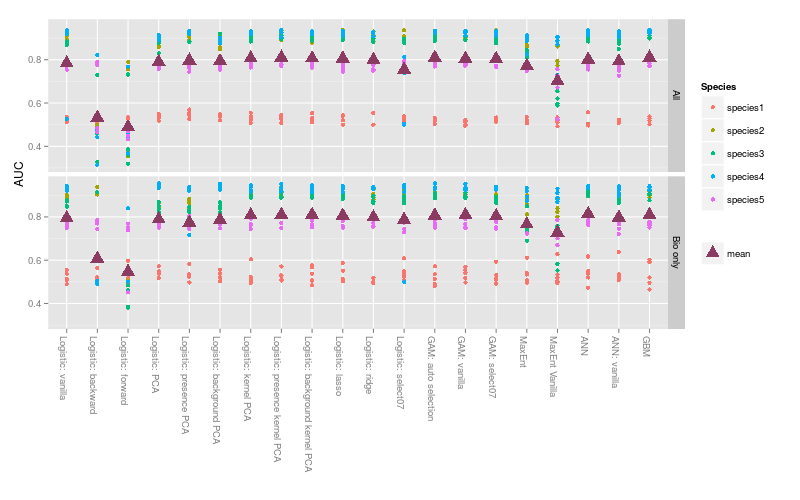
\includegraphics[scale=0.70]{Plots/SimulationAUC.png}
}
\caption{\label{fig:AUCSimulation}AUC values of the different classifiers fitted on the simulated data.}
\end{figure}


\begin{figure}[!htb]
\center
\makebox[\textwidth][c]{%
	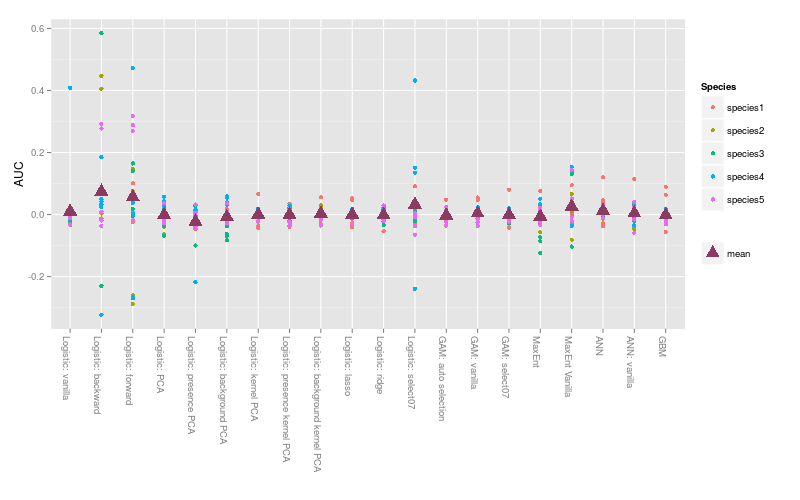
\includegraphics[scale=0.70]{Plots/SimulationDifference.png}
}
\caption{\label{fig:DiffSimulation}Difference between the AUC values when using all versus only the bioclimatic variables.}
\end{figure}

The mean AUCs largely confirm the conclusions made in Chapter \ref{ch:Applications}. In particular logistic regression performs quite well on its own. Techniques that allow for flexible non-linear relations tend to have the highest mean AUC. It is particularly interesting that MaxEnt, especially when the default parameters are used, performs quite badly. The penalized regression models seem approximately on par with the logistic regression model. The select07 logistic regression methods seems perform slightly worse than standard logistic regression. \\ 

When it comes to the stepwise methods the results diverge slightly from what was observed in Chapter \ref{ch:Applications}. More particularly the stepwise methods perform even worse. When all variables are considered these methods have a mean AUC around $0.5$ which is the same as one would get when a classifier that randomly labels the observations as presences or background points. \\

It is striking that there is no noticeable difference between performing (K)PCA on the predictor values corresponding to all, the presence, or the background locations. Given the way the virtual species were generated it was expected that the (K)PCA performed on the predictor values corresponding to background points would be superior. Hence, based on the mean AUC there seems to be no reason to prefer one over the other. \\

None of the methods perform significantly worse when the non-relevant, i.e.\ non-bioclimatic, variables are added. However, it seems reasonable that some models perform somewhat worse: especially logistic regression model, MaxEnt with the default parameters, and the stepwise models show quite a decrease. If a more extensive simulation study would be performed extra interest could be in these methods. \\

\begin{table}[!htb]
\makebox[\textwidth][c]{
\begin{tabular}{lcccccc}
 & \multicolumn{2}{c}{All} & \multicolumn{2}{c}{Bioclimatic} & \multicolumn{2}{c}{Difference} \\
 \cline{2-3} \cline{4-5} \cline{6-7}\\
 Method & $\hat{\tau}_{all}$ & 95\% CI  &  $\hat{\tau}_{bio}$ & 95\% CI &  $\hat{\tau}_{bio} - \hat{\tau}_{all}$ & 95\% CI \\

\midrule
Logistic: vanilla                 & 0.081 &  [0.009; 0.140] & 0.015  & [0.009; 0.022] & -0.066 &  [-0.130; 0.012]   \\ 
Logistic: backward                & 0.131 &  [0.067; 0.173] & 0.134  & [0.017; 0.198] & 0.003  &  [-0.143; 0.104]   \\
Logistic: forward                 & 0.143 &  [0.071; 0.190] & 0.096  & [0.037; 0.133] & -0.047 &  [-0.137; 0.041]   \\
Logistic: PCA                     & 0.021 &  [0.012; 0.030] & 0.018  & [0.013; 0.022] & -0.003 &  [-0.011; 0.007]   \\
Logistic: presence PCA            & 0.024 &  [0.012; 0.034] & 0.048  & [0.021; 0.076] & 0.024  &  [-0.008; 0.061]   \\
Logistic: background PCA          & 0.017 &  [0.012; 0.023] & 0.018  & [0.014; 0.021] & 0.001  &  [-0.008; 0.007]   \\ 
Logistic: kernel PCA              & 0.012 &  [0.008; 0.015] & 0.024  & [0.013; 0.035] & 0.012  &  [0.004; 0.020]   \\ 
Logistic: presence kernel PCA     & 0.014 &  [0.010; 0.017] & 0.018  & [0.014; 0.022] & 0.005  &  [0.000; 0.009]   \\ 
Logistic: background kernel PCA   & 0.013 &  [0.009; 0.017] & 0.022  & [0.013; 0.032] & 0.009  &  [0.001; 0.017]   \\ 
Logistic: lasso                   & 0.014 &  [0.010; 0.018] & 0.021  & [0.011; 0.030] & 0.006  &  [0.000; 0.013]   \\ 
Logistic: ridge                   & 0.016 &  [0.011; 0.021] & 0.015  & [0.010; 0.019] & -0.001 &  [-0.008; 0.004]   \\ 
Logistic: select07                & 0.068 &  [0.008; 0.117] & 0.090  & [0.018; 0.152] & 0.022  &  [0.004; 0.035]   \\ 
GAM: auto selection               & 0.011 &  [0.008; 0.013] & 0.020  & [0.011; 0.030] & 0.009  &  [0.000; 0.019]   \\ 
GAM: vanilla                      & 0.010 &  [0.008; 0.012] & 0.018  & [0.011; 0.025] & 0.008  &  [0.000; 0.014]   \\ 
GAM: select07                     & 0.011 &  [0.008; 0.013] & 0.021  & [0.011; 0.031] & 0.010  &  [0.000; 0.022]   \\ 
MaxEnt                            & 0.023 &  [0.016; 0.030] & 0.039  & [0.025; 0.050] & 0.015  &  [-0.001; 0.029]   \\
MaxEnt Vanilla                    & 0.062 &  [0.038; 0.081] & 0.062  & [0.039; 0.083] & 0.000  &  [-0.036; 0.036]   \\
ANN                               & 0.016 &  [0.010; 0.022] & 0.025  & [0.008; 0.041] & 0.009  &  [-0.002; 0.020]   \\
ANN: vanilla                      & 0.016 &  [0.011; 0.020] & 0.029  & [0.015; 0.043] & 0.013  &  [-0.003; 0.031]   \\
GBM                               & 0.012 &  [0.008; 0.015] & 0.029  & [0.010; 0.047] & 0.017  &  [-0.002; 0.035]   \\
\bottomrule
\end{tabular}}
\caption{\label{tab:SDSimulation}Estimates and bootstrapped confidence intervals of the standard deviation $\tau$.}
\end{table}

An inspection of Table \ref{tab:SDSimulation} indicates roughly that $\tau$ shows roughly the same trends as those observed in Chapter \ref{ch:Applications}. First of all the logistic regression model is quite stable when only the bioclimatic variables are considered. Once extra redundant variables are added there is a large increase in the SD. However, $0$ is included in the $95$\% CI so rigorously we cannot conclude that the SD increases. The other methods seem quite stable, which since variable selection techniques are added is to some extent what is expected. Note that $8$ of the $95$\% CI only include positive values, this would lead to the conclusion that including irrelevant variables improves the classifiers. Of course this is non-sensical and this behaviour can likely be related to the underestimation of the variance in the bootstrap procedure, see Section \ref{sec:Estimators}. \\

Just as for the mean AUC the methods that allow for flexible non-linear relations tend 
to perform the best, i.e.\ have the lowest $\hat{\tau}$ vales. Furthermore, the MaxEnt implementation that uses the default parameters has quite a high $\hat{\tau}$ and also its $95$\% CI includes relatively high values. The penalized regression methods perform quite well. In particular when the only the bioclimatic variables are considered their SD is on par with the SD of logistic regression. When all the variables are considered the SD, unlike what was the case for logistic regression, stays stable. The no influential trend is seen when the (K)PCA is performed on the different observations. Hence again there seems to be no effect of the presence vs background location. Finally, both stepwise methods are the worst methods, i.e.\ most variable, of the methods considered. The select07 method combined with logistic regression seems quite variable, this is not completely in line with the results of Section \ref{sec:POData}.


\section{Conclusion}







% backmater => mainly references
\backmatter
\printbibliography[heading=bibnumbered]
\cleardoublepage


\includepdf[pages={1}]{Cover/BackPage.pdf}
\end{document}
